\documentclass[UTF8,fontset=fandol,10pt,a4paper,landscape]{ctexart}
\usepackage[margin=18mm,headheight=16pt,headsep=5mm,footskip=9mm]{geometry}
\usepackage{amsmath,booktabs,array,xcolor,hyperref,tikz,pgfplots,fancyhdr}
\pgfplotsset{compat=1.18}
\definecolor{ink}{HTML}{20324A}
\definecolor{teal}{HTML}{008B83}
\definecolor{missing}{HTML}{D9DFE6}
\definecolor{land}{HTML}{E2E9DD}
\hypersetup{unicode=true,colorlinks=true,linkcolor=teal,urlcolor=teal,pdftitle={Singapore Rainfall 2017--2024: Exploration and Prediction},pdfauthor={Project group (Codex assistance)}}
\ctexset{section={format=\Large\bfseries\color{teal}}}
\pagestyle{fancy}\fancyhf{}
\fancyhead[L]{\small Singapore rainfall 2017--2024 / Tasks 1 and 2}
\fancyhead[R]{\small Technical report (English)}
\fancyfoot[L]{\footnotesize 9 October 2026 / Empirical analysis and prediction}
\fancyfoot[R]{\footnotesize\thepage}
\renewcommand{\headrulewidth}{.3pt}
\renewcommand{\arraystretch}{1.15}
\setlength{\parskip}{5pt}\setlength{\parindent}{0pt}
\pgfplotsset{reportaxis/.style={font=\footnotesize,grid=major,grid style={gray!15},axis line style={gray!60},tick style={gray!60},label style={font=\footnotesize},title style={font=\small},legend style={font=\scriptsize},/pgf/number format/1000 sep={}}}
\begin{document}
{\LARGE\bfseries\color{ink} Singapore rainfall: temporal-spatial patterns and prediction}\par
{\large Tasks 1 and 2: Spark exploration and probability prediction, 2017--2024}\par
\vspace{2mm}

\textbf{Group members.} Pan Yuxiang, Hou Jiacheng, Wu Jiarui.

\textbf{Study objectives.} Using Singapore rainfall observations from 2017--2024, we analyse temporal and spatial patterns and develop models to predict the probability that station rainfall accumulated over the next 30 minutes exceeds a given threshold.

\textbf{Data and methods.} The eight NEA / data.gov.sg annual datasets contain 48,538,713 source records and 48,538,627 unique valid observations from 91 station IDs. Spark performs full-data cleaning and aggregation. Annual comparisons use 21 stable stations to reduce changes caused by the monitoring network.

\textbf{Main findings.} Of all valid five-minute observations, 97.08\% are dry. Eligible diurnal samples show the highest rain frequency at 16:00--17:00 Singapore time. Available-year monthly averages have the highest frequency in November and the lowest in July, with varying eligible years and stations. In the fixed panel, duration-normalized rainfall is lowest in 2019 and highest in 2021. Nearby stations generally have more strongly correlated daily rainfall; eight years alone do not establish long-term climate change.
\begin{center}\begin{tabular}{rrrrr}
\toprule
Year & Rain / observed 24h (mm) & Wet frequency (\%) & Wet-interval intensity (mm/5min) & Mean coverage (\%)\\\midrule
2017 & 6.85 & 2.85 & 0.833 & 94.6\\
2018 & 7.10 & 2.90 & 0.840 & 82.9\\
2019 & 4.81 & 1.97 & 0.841 & 94.7\\
2020 & 7.40 & 2.92 & 0.877 & 95.3\\
2021 & 7.84 & 3.04 & 0.895 & 97.8\\
2022 & 7.71 & 3.08 & 0.868 & 99.0\\
2023 & 7.52 & 3.16 & 0.824 & 95.2\\
2024 & 7.11 & 3.01 & 0.819 & 95.6\\
\bottomrule\end{tabular}\end{center}
\noindent Each year in this table uses the same 21 stations, with equal station weights. Duration-normalized rainfall is neither an official annual total nor an actual daily total. Eligible monthly and hourly samples can vary.\clearpage\section*{1. Data sources, fields and cleaning}

\textbf{Sources and fields.} Records contain observation and update timestamps, station ID/name/device ID, coordinates, reading update timestamp, rainfall amount, type, unit and date fields. There are no temperature, humidity or wind observations. API previews identify fields and annual IDs; weather findings come from the complete annual files.

\textbf{Data checks.} After downloading complete annual CSV files, we reconcile Spark input row counts with annual API metadata and check duplicate observations, timestamp alignment and rainfall values.

\textbf{Cleaning.} Spark parses timestamps in Asia/Singapore. It accepts finite, nonnegative mm readings with the expected five-minute type and valid station ID, timestamp and CSV record. Timestamps are aligned only if within two seconds of the five-minute grid; original epochs are retained. Station-time duplicates use the latest reading update, then deterministic tie-breakers. Combined annual data are checked again for cross-file duplicates.
\begin{center}\begin{tabular}{rrrrrr}
\toprule
Year & Source rows & Duplicates removed & Off-grid over 2 s & Negative readings & Stations\\\midrule
2017 & 5,256,106 & 86 & 0 & 0 & 62\\
2018 & 4,594,246 & 0 & 0 & 0 & 56\\
2019 & 5,026,862 & 0 & 0 & 0 & 54\\
2020 & 6,334,473 & 0 & 0 & 0 & 80\\
2021 & 7,044,646 & 0 & 0 & 0 & 76\\
2022 & 7,133,230 & 0 & 0 & 0 & 72\\
2023 & 6,742,890 & 0 & 0 & 0 & 74\\
2024 & 6,406,260 & 0 & 0 & 0 & 70\\
\bottomrule\end{tabular}\end{center}

\textbf{Cleaning results.} All 86 duplicate records occur in 2017. The eight years contain no negative rainfall, timestamps more than two seconds from the five-minute grid, or cross-file duplicates. Missing intervals are not counted as zero rainfall. Additional screening of readings above 50 mm/5min identifies none.

\clearpage\section*{2. Metrics and comparable samples}
For a station and time period, let $N$ be the number of valid observations, $r_i\geq0$ the rainfall amount, $W=\sum_i\mathbf{1}(r_i>0)$ the number of wet intervals, and $E$ the expected calendar slots. We use:
\begin{align*}
\text{Coverage} &= N/E,\qquad E=288\times\text{calendar days},\\
\text{Wet frequency (\%)} &=100W/N,\\
\text{Wet-interval intensity (mm/5min)} &=\sum_i r_i/W\quad(W>0),\\
\text{Rain / observed 24h (mm)} &=288\sum_i r_i/N.
\end{align*}
Calendar denominators handle leap years. Low coverage can reflect a station operating for only part of a year. Intensity averages wet intervals only. For one station and period, normalized rainfall equals $288\times\text{frequency}/100\times\text{wet-interval intensity}$. This product generally does not hold after separate station averaging. Normalized rainfall is not an official daily or annual total and does not reconstruct missed storms.

\textbf{Fixed annual panel.} Of 91 station IDs across eight years, 21 satisfy all criteria: observations in every year, annual coverage of at least 80\% in each year, and latitude/longitude spans no larger than $0.005^\circ$. The other 70 are excluded only from fixed-panel annual comparisons; their valid observations were not deleted during cleaning. The 21 stations receive equal weights. The next page lists the station scope for each analysis.

\textbf{Monthly and diurnal samples.} Figures 2 and 4 further screen sufficiently complete months or hourly strata from the 21-station pool. Monthly summaries average stations equally, then available years equally. Each eligible year-month has 17--21 stations, and each month has 6--8 available years. Requiring the same station-month to qualify in all eight years leaves only May, June, July, September, October and December, used as an additional comparison.

\textbf{Spatial samples.} Figure 1 uses 2024, which has 70 stations. Of these, 56 have annual coverage of at least 90\% and enter map colouring; the other 14 are shown in grey. Figure 5 uses daily totals from the fixed 21 stations, requiring at least 95\% daily coverage and 365 common valid days per pair. The 80\%, 90\% and 95\% completeness thresholds are project choices.

\clearpage\section*{3. Computing environment and station scope}

\textbf{Computing environment.} Task 1 runs on an Apple Silicon Mac with 10 logical CPUs, 16 GiB RAM, macOS 26.5.2 ARM64, Python 3.12.14, Java Temurin 17.0.20.1+1 and Spark 3.5.8. Task 2 runs on gpushare with Python 3.11.10, Azul Zulu Java 17.0.20.1, Spark 3.5.8 and XGBoost 3.2.0. The gpushare container quota is 42 CPUs and about 667.68 GiB RAM; full-feature model training uses 20 CPUs and a 6 GiB default driver heap.

\textbf{Spark configuration and responsibilities.} Task 1 and the initial feature-group comparisons use single-machine \texttt{local[2]}. Full-feature model comparison and evaluation use \texttt{local[20]}, 80 shuffle partitions and default parallelism 20. XGBoost uses two workers with ten CPUs per task. Experiments run sequentially at low priority without a GPU. Spark DataFrame/SQL and windows process full-data cleaning, aggregation, labels and features; Spark ML pipelines train and evaluate models. Ordinary phases use a 6 GiB Java heap and a 12 GiB process-tree stop limit. XGBoost fitting and evaluation have a 24 GiB process-tree limit.

\textbf{Analysis samples.} Station scope and completeness criteria are chosen according to the comparison, as summarized below.
\begin{center}\begin{tabular}{p{7.0cm}p{6.8cm}p{10.5cm}}
\toprule
Analysis & Station scope & Screening rule\\\midrule
Figure 1: 2024 station map & 56 of 70 stations that year & Annual coverage $\geq90\%$; 14 shown in grey\\
Figure 2: monthly patterns & Eligible subsets of the fixed 21 & 17--21 stations per eligible year-month\\
Figure 3: annual changes & The same 21 stations & Other 70 excluded from this comparison only\\
Figure 4: diurnal patterns & Eligible strata of the fixed 21 & Year-month-hour coverage $\geq80\%$\\
Figure 5: distance and correlation & Fixed 21 stations; 210 pairs & Daily coverage $\geq95\%$; $\geq365$ shared days\\
Figure 6 left: wet amounts & All 91 stations across eight years & Wet five-minute observations only\\
Figure 6 middle/right: exceedance and persistence & Valid 2024 observations from all 70 stations & Six complete future slots or two adjacent slots\\
\bottomrule\end{tabular}\end{center}

\textbf{Cleaning checks.} Source row counts match API counts; 86 duplicate records were removed, and missing slots are not zero-filled. The overall dry fraction uses all 91 stations, rather than only the 21-station panel.

\clearpage\section*{Figure 1: Station rainfall maps in 2024}

\begin{center}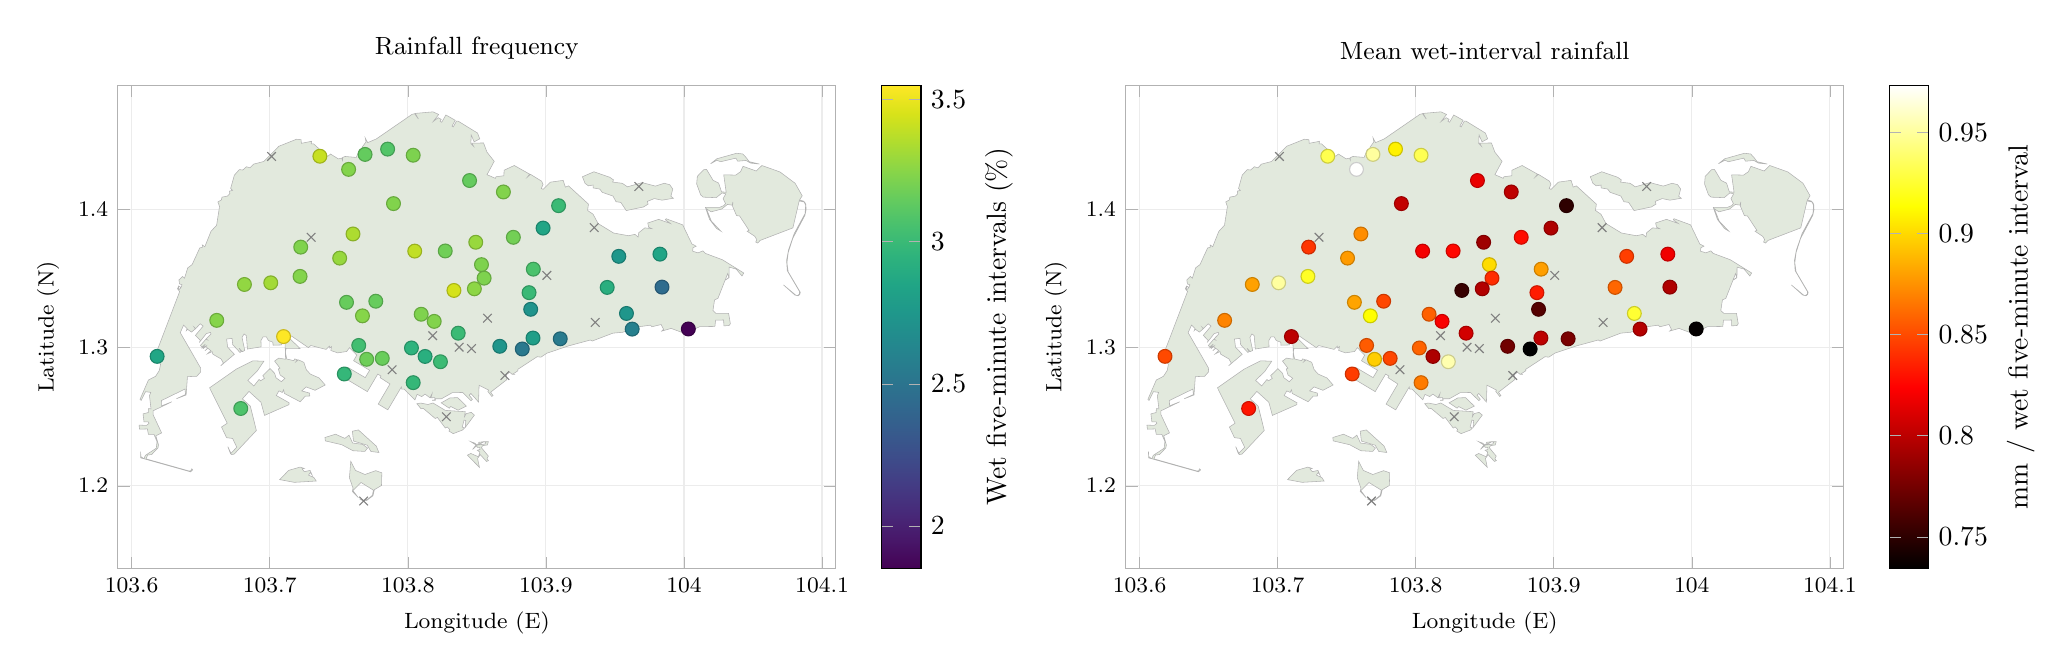
\begin{tikzpicture}
\begin{axis}[reportaxis,at={(0.0cm,0)},anchor=south west,width=10.7cm,height=8cm,title={Rainfall frequency},xlabel={Longitude (E)},ylabel={Latitude (N)},xmin=103.59,xmax=104.11,ymin=1.14,ymax=1.49,xtick={103.6,103.7,103.8,103.9,104.0,104.1},scaled ticks=false,axis equal image,point meta min=1.8499486,point meta max=3.5497582,colormap/viridis,colorbar,colorbar style={ylabel={Wet five-minute intervals (\%)}}]
\path[fill=land,draw=gray!60,line width=.2pt] (axis cs:103.7218714,1.2135462) -- (axis cs:103.7136853,1.2111756) -- (axis cs:103.7071836,1.2044931) -- (axis cs:103.7178159,1.2025194) -- (axis cs:103.7336516,1.2034740) -- (axis cs:103.7320316,1.2059304) -- (axis cs:103.7280932,1.2077765) -- (axis cs:103.7293708,1.2096419) -- (axis cs:103.7306401,1.2078811) -- (axis cs:103.7292099,1.2111542) -- (axis cs:103.7250955,1.2102398) -- (axis cs:103.7234225,1.2122353) -- (axis cs:103.7249692,1.2126089) -- (axis cs:103.7218714,1.2135462) -- cycle;
\path[fill=land,draw=gray!60,line width=.2pt] (axis cs:103.7620320,1.2111744) -- (axis cs:103.7586846,1.2177819) -- (axis cs:103.7576868,1.2058326) -- (axis cs:103.7603261,1.1982919) -- (axis cs:103.7598326,1.1959214) -- (axis cs:103.7641456,1.1914377) -- (axis cs:103.7602617,1.1965328) -- (axis cs:103.7661519,1.2024002) -- (axis cs:103.7750461,1.1968760) -- (axis cs:103.7743916,1.1931754) -- (axis cs:103.7711944,1.1905474) -- (axis cs:103.7680509,1.1895820) -- (axis cs:103.7649502,1.1905688) -- (axis cs:103.7676539,1.1891100) -- (axis cs:103.7702181,1.1893889) -- (axis cs:103.7746920,1.1927249) -- (axis cs:103.7757971,1.1971978) -- (axis cs:103.7809255,1.2002549) -- (axis cs:103.7811830,1.2094260) -- (axis cs:103.7767412,1.2109813) -- (axis cs:103.7689521,1.2082032) -- (axis cs:103.7620320,1.2111744) -- cycle;
\path[fill=land,draw=gray!60,line width=.2pt] (axis cs:103.8486849,1.2308515) -- (axis cs:103.8455629,1.2319805) -- (axis cs:103.8494038,1.2295376) -- (axis cs:103.8469575,1.2263895) -- (axis cs:103.8500045,1.2291408) -- (axis cs:103.8502351,1.2278215) -- (axis cs:103.8521824,1.2278965) -- (axis cs:103.8522575,1.2262500) -- (axis cs:103.8502724,1.2257929) -- (axis cs:103.8521355,1.2244850) -- (axis cs:103.8512222,1.2209995) -- (axis cs:103.8456362,1.2234323) -- (axis cs:103.8431678,1.2221753) -- (axis cs:103.8518459,1.2133951) -- (axis cs:103.8505147,1.2198074) -- (axis cs:103.8524453,1.2225870) -- (axis cs:103.8570170,1.2176462) -- (axis cs:103.8584159,1.2182431) -- (axis cs:103.8573537,1.2194981) -- (axis cs:103.8583086,1.2215575) -- (axis cs:103.8533371,1.2275506) -- (axis cs:103.8541599,1.2291208) -- (axis cs:103.8575994,1.2295976) -- (axis cs:103.8583408,1.2320265) -- (axis cs:103.8552723,1.2319299) -- (axis cs:103.8565583,1.2314090) -- (axis cs:103.8557012,1.2302183) -- (axis cs:103.8510722,1.2296501) -- (axis cs:103.8551221,1.2319407) -- (axis cs:103.8513256,1.2315290) -- (axis cs:103.8517156,1.2306119) -- (axis cs:103.8495406,1.2296934) -- (axis cs:103.8486849,1.2308515) -- cycle;
\path[fill=land,draw=gray!60,line width=.2pt] (axis cs:103.7476729,1.2373733) -- (axis cs:103.7399913,1.2350135) -- (axis cs:103.7402595,1.2325411) -- (axis cs:103.7521522,1.2297737) -- (axis cs:103.7602578,1.2254295) -- (axis cs:103.7688702,1.2248936) -- (axis cs:103.7708464,1.2273636) -- (axis cs:103.7672798,1.2300418) -- (axis cs:103.7600003,1.2309965) -- (axis cs:103.7573878,1.2366868) -- (axis cs:103.7543999,1.2343592) -- (axis cs:103.7476729,1.2373733) -- cycle;
\path[fill=land,draw=gray!60,line width=.2pt] (axis cs:103.7642004,1.2404758) -- (axis cs:103.7598506,1.2395345) -- (axis cs:103.7606730,1.2324175) -- (axis cs:103.7706812,1.2293918) -- (axis cs:103.7732518,1.2248868) -- (axis cs:103.7790706,1.2241368) -- (axis cs:103.7771103,1.2288073) -- (axis cs:103.7642004,1.2404758) -- cycle;
\path[fill=land,draw=gray!60,line width=.2pt] (axis cs:103.8092243,1.2599535) -- (axis cs:103.8065464,1.2594643) -- (axis cs:103.8095960,1.2558145) -- (axis cs:103.8111558,1.2561021) -- (axis cs:103.8198502,1.2487724) -- (axis cs:103.8214162,1.2494962) -- (axis cs:103.8271395,1.2418785) -- (axis cs:103.8285563,1.2426188) -- (axis cs:103.8303607,1.2408087) -- (axis cs:103.8298058,1.2396090) -- (axis cs:103.8329043,1.2377975) -- (axis cs:103.8397613,1.2404646) -- (axis cs:103.8409947,1.2419423) -- (axis cs:103.8394128,1.2424937) -- (axis cs:103.8407222,1.2476237) -- (axis cs:103.8419874,1.2473115) -- (axis cs:103.8415699,1.2422848) -- (axis cs:103.8482440,1.2512187) -- (axis cs:103.8458752,1.2532370) -- (axis cs:103.8422471,1.2522502) -- (axis cs:103.8410200,1.2500391) -- (axis cs:103.8416019,1.2536860) -- (axis cs:103.8271716,1.2546277) -- (axis cs:103.8182014,1.2599936) -- (axis cs:103.8145996,1.2589044) -- (axis cs:103.8092243,1.2599535) -- cycle;
\path[fill=land,draw=gray!60,line width=.2pt] (axis cs:103.8424306,1.2577463) -- (axis cs:103.8360929,1.2639018) -- (axis cs:103.8304601,1.2636316) -- (axis cs:103.8241852,1.2600970) -- (axis cs:103.8299800,1.2562194) -- (axis cs:103.8310878,1.2574185) -- (axis cs:103.8363807,1.2547801) -- (axis cs:103.8424306,1.2577463) -- cycle;
\path[fill=land,draw=gray!60,line width=.2pt] (axis cs:103.7122938,1.2918543) -- (axis cs:103.7113394,1.2966262) -- (axis cs:103.7112700,1.2917036) -- (axis cs:103.7064550,1.2924988) -- (axis cs:103.7035362,1.2903439) -- (axis cs:103.7074308,1.2852082) -- (axis cs:103.7062415,1.2846126) -- (axis cs:103.7075198,1.2802953) -- (axis cs:103.7109689,1.2778593) -- (axis cs:103.7084122,1.2753991) -- (axis cs:103.7045050,1.2782934) -- (axis cs:103.7035402,1.2815012) -- (axis cs:103.7002118,1.2849020) -- (axis cs:103.6949663,1.2797840) -- (axis cs:103.6961704,1.2778236) -- (axis cs:103.6933610,1.2760638) -- (axis cs:103.6922496,1.2770209) -- (axis cs:103.6884616,1.2723096) -- (axis cs:103.6840829,1.2763658) -- (axis cs:103.6907662,1.2829109) -- (axis cs:103.6957243,1.2902193) -- (axis cs:103.6877922,1.2905557) -- (axis cs:103.6758065,1.2845554) -- (axis cs:103.6564315,1.2709859) -- (axis cs:103.6691685,1.2453464) -- (axis cs:103.6650610,1.2426035) -- (axis cs:103.6687358,1.2348759) -- (axis cs:103.6730843,1.2343241) -- (axis cs:103.6761219,1.2279306) -- (axis cs:103.6719049,1.2235569) -- (axis cs:103.6696304,1.2283746) -- (axis cs:103.6715981,1.2232104) -- (axis cs:103.6724886,1.2226752) -- (axis cs:103.6741961,1.2229573) -- (axis cs:103.6903236,1.2400948) -- (axis cs:103.6859149,1.2577423) -- (axis cs:103.6801960,1.2629621) -- (axis cs:103.6849630,1.2683900) -- (axis cs:103.6936240,1.2605314) -- (axis cs:103.6962199,1.2509973) -- (axis cs:103.7138957,1.2587851) -- (axis cs:103.7140137,1.2601302) -- (axis cs:103.7047392,1.2654164) -- (axis cs:103.7066272,1.2687675) -- (axis cs:103.7090343,1.2676348) -- (axis cs:103.7100255,1.2695463) -- (axis cs:103.7106154,1.2668796) -- (axis cs:103.7220594,1.2608872) -- (axis cs:103.7256957,1.2648956) -- (axis cs:103.7289839,1.2650838) -- (axis cs:103.7288176,1.2671400) -- (axis cs:103.7231703,1.2687536) -- (axis cs:103.7263483,1.2716416) -- (axis cs:103.7328278,1.2691965) -- (axis cs:103.7401808,1.2730367) -- (axis cs:103.7357015,1.2781600) -- (axis cs:103.7293769,1.2809212) -- (axis cs:103.7264616,1.2841474) -- (axis cs:103.7247042,1.2894169) -- (axis cs:103.7207624,1.2912551) -- (axis cs:103.7189082,1.2898277) -- (axis cs:103.7199365,1.2913215) -- (axis cs:103.7180121,1.2919348) -- (axis cs:103.7174625,1.2906332) -- (axis cs:103.7122938,1.2918543) -- cycle;
\path[fill=land,draw=gray!60,line width=.2pt] (axis cs:103.9347848,1.4274582) -- (axis cs:103.9264553,1.4238528) -- (axis cs:103.9283554,1.4190909) -- (axis cs:103.9307089,1.4172997) -- (axis cs:103.9341981,1.4178389) -- (axis cs:103.9342492,1.4157588) -- (axis cs:103.9390356,1.4149261) -- (axis cs:103.9407791,1.4126004) -- (axis cs:103.9486000,1.4098409) -- (axis cs:103.9507941,1.4057751) -- (axis cs:103.9542260,1.4052956) -- (axis cs:103.9581645,1.3993755) -- (axis cs:103.9706674,1.4019552) -- (axis cs:103.9740223,1.4040136) -- (axis cs:103.9735180,1.4060345) -- (axis cs:103.9785241,1.4080405) -- (axis cs:103.9841158,1.4068838) -- (axis cs:103.9923787,1.4082651) -- (axis cs:103.9905172,1.4096951) -- (axis cs:103.9918896,1.4149416) -- (axis cs:103.9896761,1.4181120) -- (axis cs:103.9857025,1.4191236) -- (axis cs:103.9793108,1.4170770) -- (axis cs:103.9697473,1.4195916) -- (axis cs:103.9590472,1.4165605) -- (axis cs:103.9553897,1.4190717) -- (axis cs:103.9483697,1.4200054) -- (axis cs:103.9489322,1.4215867) -- (axis cs:103.9462272,1.4234840) -- (axis cs:103.9347848,1.4274582) -- cycle;
\path[fill=land,draw=gray!60,line width=.2pt] (axis cs:104.0564354,1.4319912) -- (axis cs:104.0523476,1.4280138) -- (axis cs:104.0427989,1.4314030) -- (axis cs:104.0409428,1.4274560) -- (axis cs:104.0374559,1.4250428) -- (axis cs:104.0287978,1.4252466) -- (axis cs:104.0305817,1.4126055) -- (axis cs:104.0271586,1.4129725) -- (axis cs:104.0251277,1.4192165) -- (axis cs:104.0210703,1.4212912) -- (axis cs:104.0163225,1.4292324) -- (axis cs:104.0142840,1.4289536) -- (axis cs:104.0096920,1.4241700) -- (axis cs:104.0091985,1.4186571) -- (axis cs:104.0120539,1.4107788) -- (axis cs:104.0139554,1.4090618) -- (axis cs:104.0234255,1.4087027) -- (axis cs:104.0275088,1.4120940) -- (axis cs:104.0302569,1.4115109) -- (axis cs:104.0283552,1.4079222) -- (axis cs:104.0301364,1.4044494) -- (axis cs:104.0288269,1.4029269) -- (axis cs:104.0256775,1.4016190) -- (axis cs:104.0155382,1.4016329) -- (axis cs:104.0185101,1.3929676) -- (axis cs:104.0236170,1.3863805) -- (axis cs:104.0267373,1.3844740) -- (axis cs:104.0198171,1.3917600) -- (axis cs:104.0162843,1.4006832) -- (axis cs:104.0196325,1.3984322) -- (axis cs:104.0272133,1.4004182) -- (axis cs:104.0315136,1.4038121) -- (axis cs:104.0348994,1.4032595) -- (axis cs:104.0354552,1.4056401) -- (axis cs:104.0351708,1.4025176) -- (axis cs:104.0380675,1.3956961) -- (axis cs:104.0402798,1.3954418) -- (axis cs:104.0471225,1.3850148) -- (axis cs:104.0457937,1.3843823) -- (axis cs:104.0513332,1.3806463) -- (axis cs:104.0527138,1.3783713) -- (axis cs:104.0519710,1.3765520) -- (axis cs:104.0534400,1.3758529) -- (axis cs:104.0551621,1.3777270) -- (axis cs:104.0788833,1.3868077) -- (axis cs:104.0834592,1.4063608) -- (axis cs:104.0870834,1.4055086) -- (axis cs:104.0881184,1.4031815) -- (axis cs:104.0877124,1.3971833) -- (axis cs:104.0798211,1.3826473) -- (axis cs:104.0757440,1.3709126) -- (axis cs:104.0743140,1.3632571) -- (axis cs:104.0748245,1.3557917) -- (axis cs:104.0837155,1.3406798) -- (axis cs:104.0836389,1.3387925) -- (axis cs:104.0821521,1.3378084) -- (axis cs:104.0809936,1.3380943) -- (axis cs:104.0721000,1.3454826) -- (axis cs:104.0803605,1.3381498) -- (axis cs:104.0826739,1.3376214) -- (axis cs:104.0839005,1.3385883) -- (axis cs:104.0842330,1.3401989) -- (axis cs:104.0754939,1.3550027) -- (axis cs:104.0745771,1.3615437) -- (axis cs:104.0755149,1.3689862) -- (axis cs:104.0787758,1.3791644) -- (axis cs:104.0876107,1.3959251) -- (axis cs:104.0884735,1.3999567) -- (axis cs:104.0882509,1.4039273) -- (axis cs:104.0875567,1.4052694) -- (axis cs:104.0864177,1.4062781) -- (axis cs:104.0837021,1.4070227) -- (axis cs:104.0856392,1.4100485) -- (axis cs:104.0804893,1.4191545) -- (axis cs:104.0694923,1.4273488) -- (axis cs:104.0564354,1.4319912) -- cycle;
\path[fill=land,draw=gray!60,line width=.2pt] (axis cs:104.0450543,1.4377270) -- (axis cs:104.0426081,1.4403440) -- (axis cs:104.0380805,1.4408589) -- (axis cs:104.0238326,1.4368690) -- (axis cs:104.0192836,1.4332652) -- (axis cs:104.0238258,1.4357786) -- (axis cs:104.0265712,1.4347315) -- (axis cs:104.0376514,1.4373409) -- (axis cs:104.0388559,1.4351089) -- (axis cs:104.0449187,1.4356701) -- (axis cs:104.0482086,1.4337372) -- (axis cs:104.0546221,1.4330547) -- (axis cs:104.0472859,1.4347453) -- (axis cs:104.0450543,1.4377270) -- cycle;
\path[fill=land,draw=gray!60,line width=.2pt] (axis cs:103.8182588,1.4708518) -- (axis cs:103.8053927,1.4697255) -- (axis cs:103.8076479,1.4656682) -- (axis cs:103.8049642,1.4695130) -- (axis cs:103.8030522,1.4690433) -- (axis cs:103.7771316,1.4511975) -- (axis cs:103.7709060,1.4485682) -- (axis cs:103.7691570,1.4519377) -- (axis cs:103.7697223,1.4491016) -- (axis cs:103.7668745,1.4452242) -- (axis cs:103.7676612,1.4429178) -- (axis cs:103.7662095,1.4412665) -- (axis cs:103.7670850,1.4436947) -- (axis cs:103.7649993,1.4437119) -- (axis cs:103.7626974,1.4378483) -- (axis cs:103.7545774,1.4385362) -- (axis cs:103.7526606,1.4377275) -- (axis cs:103.7527188,1.4357764) -- (axis cs:103.7520769,1.4373700) -- (axis cs:103.7496835,1.4367728) -- (axis cs:103.7440225,1.4402920) -- (axis cs:103.7423426,1.4388867) -- (axis cs:103.7385122,1.4388929) -- (axis cs:103.7376659,1.4405359) -- (axis cs:103.7365907,1.4387268) -- (axis cs:103.7372160,1.4427400) -- (axis cs:103.7318557,1.4475852) -- (axis cs:103.7300113,1.4476237) -- (axis cs:103.7303212,1.4495208) -- (axis cs:103.7229053,1.4480731) -- (axis cs:103.7226475,1.4506971) -- (axis cs:103.7193476,1.4510112) -- (axis cs:103.7066255,1.4459478) -- (axis cs:103.6956326,1.4348973) -- (axis cs:103.6882809,1.4329826) -- (axis cs:103.6857365,1.4303318) -- (axis cs:103.6831155,1.4310961) -- (axis cs:103.6804816,1.4287252) -- (axis cs:103.6780030,1.4290148) -- (axis cs:103.6743687,1.4250127) -- (axis cs:103.6716769,1.4153383) -- (axis cs:103.6730173,1.4139789) -- (axis cs:103.6708347,1.4134335) -- (axis cs:103.6710756,1.4115459) -- (axis cs:103.6694408,1.4098629) -- (axis cs:103.6653997,1.4090807) -- (axis cs:103.6650129,1.4070751) -- (axis cs:103.6624333,1.4056023) -- (axis cs:103.6636304,1.4022810) -- (axis cs:103.6615174,1.3887099) -- (axis cs:103.6574265,1.3843114) -- (axis cs:103.6529800,1.3731525) -- (axis cs:103.6511133,1.3744640) -- (axis cs:103.6512697,1.3728335) -- (axis cs:103.6493014,1.3722583) -- (axis cs:103.6437619,1.3602143) -- (axis cs:103.6405957,1.3578450) -- (axis cs:103.6382792,1.3503882) -- (axis cs:103.6368028,1.3516427) -- (axis cs:103.6342209,1.3491005) -- (axis cs:103.6347014,1.3461831) -- (axis cs:103.6364706,1.3456102) -- (axis cs:103.6356485,1.3435165) -- (axis cs:103.6343676,1.3446189) -- (axis cs:103.6355865,1.3434299) -- (axis cs:103.6341661,1.3419075) -- (axis cs:103.6339614,1.3444615) -- (axis cs:103.6331867,1.3427146) -- (axis cs:103.6347608,1.3407358) -- (axis cs:103.6181088,1.2970886) -- (axis cs:103.6174833,1.2935735) -- (axis cs:103.6209090,1.2879076) -- (axis cs:103.6200196,1.2835196) -- (axis cs:103.6173097,1.2793141) -- (axis cs:103.6121369,1.2766392) -- (axis cs:103.6060390,1.2626124) -- (axis cs:103.6068705,1.2618638) -- (axis cs:103.6100054,1.2681708) -- (axis cs:103.6138313,1.2676795) -- (axis cs:103.6128858,1.2652678) -- (axis cs:103.6140041,1.2556897) -- (axis cs:103.6121941,1.2559461) -- (axis cs:103.6119779,1.2530555) -- (axis cs:103.6082329,1.2521227) -- (axis cs:103.6089237,1.2463372) -- (axis cs:103.6120770,1.2463400) -- (axis cs:103.6125468,1.2452612) -- (axis cs:103.6107272,1.2437509) -- (axis cs:103.6053499,1.2439697) -- (axis cs:103.6057232,1.2409921) -- (axis cs:103.6113573,1.2412103) -- (axis cs:103.6121061,1.2373263) -- (axis cs:103.6161606,1.2371965) -- (axis cs:103.6183578,1.2320725) -- (axis cs:103.6178203,1.2272264) -- (axis cs:103.6099411,1.2220852) -- (axis cs:103.6088671,1.2196085) -- (axis cs:103.6066591,1.2211520) -- (axis cs:103.6064638,1.2248430) -- (axis cs:103.6065411,1.2202542) -- (axis cs:103.6426458,1.2101274) -- (axis cs:103.6442068,1.2115390) -- (axis cs:103.6435073,1.2123360) -- (axis cs:103.6427895,1.2108311) -- (axis cs:103.6411148,1.2108740) -- (axis cs:103.6104088,1.2195195) -- (axis cs:103.6115708,1.2222890) -- (axis cs:103.6144933,1.2227057) -- (axis cs:103.6190107,1.2274082) -- (axis cs:103.6194254,1.2295819) -- (axis cs:103.6175070,1.2362590) -- (axis cs:103.6216838,1.2383153) -- (axis cs:103.6154729,1.2515848) -- (axis cs:103.6154707,1.2543178) -- (axis cs:103.6290759,1.2608641) -- (axis cs:103.6217460,1.2579412) -- (axis cs:103.6215926,1.2617747) -- (axis cs:103.6386525,1.2701036) -- (axis cs:103.6389776,1.2661081) -- (axis cs:103.6324030,1.2630662) -- (axis cs:103.6394261,1.2658035) -- (axis cs:103.6404044,1.2790737) -- (axis cs:103.6471602,1.2793465) -- (axis cs:103.6500050,1.2825393) -- (axis cs:103.6498825,1.2854139) -- (axis cs:103.6351888,1.3109266) -- (axis cs:103.6376362,1.3164053) -- (axis cs:103.6401457,1.3139256) -- (axis cs:103.6396284,1.3124489) -- (axis cs:103.6404806,1.3133562) -- (axis cs:103.6432811,1.3113296) -- (axis cs:103.6461014,1.3136691) -- (axis cs:103.6453654,1.3147587) -- (axis cs:103.6463112,1.3138842) -- (axis cs:103.6496585,1.3173514) -- (axis cs:103.6517879,1.3156879) -- (axis cs:103.6461727,1.3089633) -- (axis cs:103.6497890,1.3052323) -- (axis cs:103.6489539,1.3038054) -- (axis cs:103.6540343,1.3102113) -- (axis cs:103.6570286,1.3111274) -- (axis cs:103.6574369,1.3099816) -- (axis cs:103.6540041,1.3064885) -- (axis cs:103.6547980,1.3057262) -- (axis cs:103.6537672,1.3062204) -- (axis cs:103.6498210,1.3016827) -- (axis cs:103.6508446,1.3004613) -- (axis cs:103.6533560,1.3025933) -- (axis cs:103.6512250,1.2999916) -- (axis cs:103.6538227,1.3013019) -- (axis cs:103.6517678,1.2993374) -- (axis cs:103.6537510,1.3010146) -- (axis cs:103.6549282,1.2996593) -- (axis cs:103.6530519,1.2978329) -- (axis cs:103.6551805,1.2996310) -- (axis cs:103.6573391,1.2979103) -- (axis cs:103.6549011,1.2956166) -- (axis cs:103.6582254,1.2972388) -- (axis cs:103.6587850,1.2953365) -- (axis cs:103.6647575,1.2918636) -- (axis cs:103.6664408,1.2888460) -- (axis cs:103.6644960,1.2869247) -- (axis cs:103.6743803,1.2952635) -- (axis cs:103.6695020,1.3004336) -- (axis cs:103.6687381,1.3062925) -- (axis cs:103.6727046,1.3067940) -- (axis cs:103.6732136,1.3022238) -- (axis cs:103.6784339,1.2965888) -- (axis cs:103.6793691,1.2971788) -- (axis cs:103.6778311,1.2996652) -- (axis cs:103.6801249,1.2971736) -- (axis cs:103.6819040,1.2979865) -- (axis cs:103.6799362,1.3074632) -- (axis cs:103.6813899,1.3100089) -- (axis cs:103.6830343,1.3087891) -- (axis cs:103.6838606,1.2990801) -- (axis cs:103.6937884,1.3006493) -- (axis cs:103.6936115,1.3051766) -- (axis cs:103.6951240,1.3078075) -- (axis cs:103.6975186,1.3079392) -- (axis cs:103.6989904,1.3052733) -- (axis cs:103.7022863,1.3040062) -- (axis cs:103.7023992,1.3018237) -- (axis cs:103.7086886,1.3020480) -- (axis cs:103.7083835,1.3076134) -- (axis cs:103.7099572,1.3070171) -- (axis cs:103.7108258,1.3084149) -- (axis cs:103.7113395,1.2971629) -- (axis cs:103.7118883,1.2995865) -- (axis cs:103.7219279,1.2994621) -- (axis cs:103.7146266,1.3065352) -- (axis cs:103.7125573,1.3065835) -- (axis cs:103.7127174,1.3088684) -- (axis cs:103.7158417,1.3084267) -- (axis cs:103.7279367,1.3001075) -- (axis cs:103.7297772,1.3015932) -- (axis cs:103.7408521,1.2988015) -- (axis cs:103.7432117,1.3011478) -- (axis cs:103.7434282,1.2998111) -- (axis cs:103.7447614,1.3008186) -- (axis cs:103.7442093,1.2980363) -- (axis cs:103.7492007,1.2962988) -- (axis cs:103.7557489,1.2972886) -- (axis cs:103.7577412,1.3000673) -- (axis cs:103.7630421,1.2946161) -- (axis cs:103.7607166,1.2906021) -- (axis cs:103.7723383,1.2836930) -- (axis cs:103.7691344,1.2783691) -- (axis cs:103.7564771,1.2858293) -- (axis cs:103.7530224,1.2853155) -- (axis cs:103.7501846,1.2805019) -- (axis cs:103.7706766,1.2682258) -- (axis cs:103.7782058,1.2809173) -- (axis cs:103.7805823,1.2795141) -- (axis cs:103.7799596,1.2783461) -- (axis cs:103.7870605,1.2737594) -- (axis cs:103.7785642,1.2592010) -- (axis cs:103.7855063,1.2550200) -- (axis cs:103.7953085,1.2715722) -- (axis cs:103.7955723,1.2700867) -- (axis cs:103.7973420,1.2700456) -- (axis cs:103.8051473,1.2622774) -- (axis cs:103.8067358,1.2662291) -- (axis cs:103.8100922,1.2646416) -- (axis cs:103.8124604,1.2664141) -- (axis cs:103.8160516,1.2637829) -- (axis cs:103.8175506,1.2666830) -- (axis cs:103.8167869,1.2637038) -- (axis cs:103.8194715,1.2639086) -- (axis cs:103.8197099,1.2622559) -- (axis cs:103.8176424,1.2619600) -- (axis cs:103.8198650,1.2619386) -- (axis cs:103.8199064,1.2630808) -- (axis cs:103.8244200,1.2630748) -- (axis cs:103.8321670,1.2674278) -- (axis cs:103.8396526,1.2676267) -- (axis cs:103.8457821,1.2616611) -- (axis cs:103.8467730,1.2627421) -- (axis cs:103.8444309,1.2656247) -- (axis cs:103.8456794,1.2668761) -- (axis cs:103.8512255,1.2606747) -- (axis cs:103.8516078,1.2728398) -- (axis cs:103.8584945,1.2693503) -- (axis cs:103.8579787,1.2683336) -- (axis cs:103.8608496,1.2647333) -- (axis cs:103.8617123,1.2653498) -- (axis cs:103.8599603,1.2677976) -- (axis cs:103.8716769,1.2768781) -- (axis cs:103.8714562,1.2805550) -- (axis cs:103.8737178,1.2822201) -- (axis cs:103.8757276,1.2807170) -- (axis cs:103.8776890,1.2807350) -- (axis cs:103.8758917,1.2807729) -- (axis cs:103.8797504,1.2833276) -- (axis cs:103.8796729,1.2843651) -- (axis cs:103.8936756,1.2935206) -- (axis cs:103.8963751,1.2931770) -- (axis cs:103.9007930,1.2960860) -- (axis cs:103.9165583,1.3013812) -- (axis cs:103.9321877,1.3056014) -- (axis cs:103.9335464,1.3048712) -- (axis cs:103.9485395,1.3105790) -- (axis cs:103.9557581,1.3112303) -- (axis cs:103.9631165,1.3146177) -- (axis cs:103.9757511,1.3163696) -- (axis cs:103.9767675,1.3151917) -- (axis cs:103.9834673,1.3168347) -- (axis cs:103.9852381,1.3133709) -- (axis cs:103.9839171,1.3120678) -- (axis cs:103.9906944,1.3140089) -- (axis cs:104.0006331,1.3103307) -- (axis cs:104.0114272,1.3152807) -- (axis cs:104.0224125,1.3154343) -- (axis cs:104.0229163,1.3199628) -- (axis cs:104.0287502,1.3201058) -- (axis cs:104.0288982,1.3158118) -- (axis cs:104.0327311,1.3161314) -- (axis cs:104.0335984,1.3174026) -- (axis cs:104.0323397,1.3249192) -- (axis cs:104.0231536,1.3248948) -- (axis cs:104.0209889,1.3269507) -- (axis cs:104.0221413,1.3346203) -- (axis cs:104.0246329,1.3358125) -- (axis cs:104.0316545,1.3537211) -- (axis cs:104.0325318,1.3509476) -- (axis cs:104.0301054,1.3490751) -- (axis cs:104.0326689,1.3507934) -- (axis cs:104.0327309,1.3584039) -- (axis cs:104.0378255,1.3569563) -- (axis cs:104.0420205,1.3519602) -- (axis cs:104.0433039,1.3541415) -- (axis cs:104.0278327,1.3637475) -- (axis cs:104.0155066,1.3683283) -- (axis cs:104.0137145,1.3701687) -- (axis cs:104.0101775,1.3687146) -- (axis cs:104.0062655,1.3699572) -- (axis cs:104.0065479,1.3724714) -- (axis cs:104.0088241,1.3735765) -- (axis cs:104.0057428,1.3751740) -- (axis cs:103.9990392,1.3890380) -- (axis cs:103.9870888,1.3934326) -- (axis cs:103.9864779,1.3927176) -- (axis cs:103.9901005,1.3900550) -- (axis cs:103.9816617,1.3929900) -- (axis cs:103.9737816,1.3903800) -- (axis cs:103.9744288,1.3873270) -- (axis cs:103.9766002,1.3862741) -- (axis cs:103.9716404,1.3868183) -- (axis cs:103.9672216,1.3832887) -- (axis cs:103.9667880,1.3801998) -- (axis cs:103.9644751,1.3821290) -- (axis cs:103.9598207,1.3811390) -- (axis cs:103.9490378,1.3830880) -- (axis cs:103.9377941,1.3899507) -- (axis cs:103.9341970,1.3966828) -- (axis cs:103.9301739,1.3994603) -- (axis cs:103.9308457,1.4040196) -- (axis cs:103.9163703,1.4172481) -- (axis cs:103.9140967,1.4163367) -- (axis cs:103.9125266,1.4212252) -- (axis cs:103.9032489,1.4199306) -- (axis cs:103.8980253,1.4147270) -- (axis cs:103.8966801,1.4153418) -- (axis cs:103.8979293,1.4183101) -- (axis cs:103.8969491,1.4206060) -- (axis cs:103.8888773,1.4255754) -- (axis cs:103.8865729,1.4235974) -- (axis cs:103.8881975,1.4257500) -- (axis cs:103.8770922,1.4320010) -- (axis cs:103.8697209,1.4285682) -- (axis cs:103.8695778,1.4245748) -- (axis cs:103.8639737,1.4238589) -- (axis cs:103.8634290,1.4226914) -- (axis cs:103.8573725,1.4253534) -- (axis cs:103.8625597,1.4350457) -- (axis cs:103.8573417,1.4416513) -- (axis cs:103.8548383,1.4483195) -- (axis cs:103.8464426,1.4481606) -- (axis cs:103.8476029,1.4459637) -- (axis cs:103.8456568,1.4478619) -- (axis cs:103.8458937,1.4540789) -- (axis cs:103.8480491,1.4491261) -- (axis cs:103.8520917,1.4512969) -- (axis cs:103.8504919,1.4554899) -- (axis cs:103.8364373,1.4641319) -- (axis cs:103.8352614,1.4641570) -- (axis cs:103.8329059,1.4599476) -- (axis cs:103.8319875,1.4604881) -- (axis cs:103.8343307,1.4647354) -- (axis cs:103.8275713,1.4685888) -- (axis cs:103.8245580,1.4633250) -- (axis cs:103.8233659,1.4640054) -- (axis cs:103.8241553,1.4654385) -- (axis cs:103.8220573,1.4666180) -- (axis cs:103.8184541,1.4639199) -- (axis cs:103.8223514,1.4689723) -- (axis cs:103.8182588,1.4708518) -- cycle;
\addplot[scatter,only marks,mark=*,mark size=2.5pt,scatter src=explicit,draw=white] coordinates {(103.8334000,1.3415000)[3.4435342] (103.8271000,1.3701000)[3.1824463] (103.7853800,1.4438700)[3.0918641] (103.9625000,1.3135000)[2.5892315] (103.8492000,1.3764000)[3.2890478] (103.8365000,1.3105500)[3.0057848] (103.9104000,1.3064800)[2.5503769] (103.6184300,1.2937700)[2.8535368] (103.7540000,1.2810000)[2.9783514] (103.6790000,1.2560000)[3.0748623] (103.8666000,1.3010500)[2.7376375] (103.7224400,1.3728800)[3.2260951] (103.7671400,1.3231100)[3.2437936] (103.7702000,1.2916400)[3.1747778] (103.9583600,1.3248500)[2.7414981] (104.0031700,1.3136000)[1.8499486] (103.8447200,1.4211100)[3.1501838] (103.7690400,1.4400300)[3.1479295] (103.7571100,1.4291800)[3.2347665] (103.8097000,1.3242700)[3.2224443] (103.8828900,1.2991100)[2.5328018] (103.8889900,1.3278500)[2.7249471] (103.8533500,1.3601900)[3.2208034] (103.8552600,1.3504100)[3.2212619] (103.7506500,1.3649100)[3.2874079] (103.8764300,1.3799900)[3.1883920] (103.8979700,1.3866600)[2.8519770] (103.8908800,1.3569100)[3.0669357] (103.8236400,1.2898700)[3.0123292] (103.8026400,1.2998400)[2.9495552] (103.9840900,1.3439200)[2.4448970] (103.8038900,1.2747200)[2.9807924] (103.8038900,1.4394400)[3.2163214] (103.7007300,1.3470300)[3.3176979] (103.7219500,1.3516700)[3.2341859] (103.7644400,1.3016700)[3.0342242] (103.9826000,1.3678000)[2.8477024] (103.7100000,1.3081000)[3.5497582] (103.7556000,1.3329000)[3.1560859] (103.7896200,1.4044000)[3.2294191] (103.8878000,1.3399000)[2.9989659] (103.6816600,1.3458300)[3.2741796] (103.7768000,1.3337000)[3.1556849] (103.7603000,1.3824000)[3.3426584] (103.7363000,1.4387000)[3.4082697] (103.8050000,1.3700000)[3.3929479] (103.7815000,1.2923000)[3.1618164] (103.8125000,1.2937000)[2.9195740] (103.8906700,1.3070300)[2.7997336] (103.9092000,1.4029000)[3.0049620] (103.9444000,1.3437000)[2.9166544] (103.8482000,1.3427000)[3.2600388] (103.6616200,1.3198500)[3.2422172] (103.8191000,1.3191000)[3.2326640] (103.8692200,1.4128400)[3.2314234] (103.9528000,1.3662000)[2.7463803]};
\addplot[gray,only marks,mark=x,mark size=2.2pt] coordinates {(103.9007000,1.3524000) (103.7680000,1.1890000) (103.9673000,1.4168000) (103.8703000,1.2799000) (103.7013100,1.4385400) (103.7300000,1.3800000) (103.8461000,1.2994000) (103.8180000,1.3087400) (103.8577000,1.3214000) (103.9357400,1.3183500) (103.9350000,1.3870000) (103.8279000,1.2500000) (103.8372000,1.3004000) (103.7886000,1.2841000)};
\end{axis}
\begin{axis}[reportaxis,at={(12.8cm,0)},anchor=south west,width=10.7cm,height=8cm,title={Mean wet-interval rainfall},xlabel={Longitude (E)},ylabel={Latitude (N)},xmin=103.59,xmax=104.11,ymin=1.14,ymax=1.49,xtick={103.6,103.7,103.8,103.9,104.0,104.1},scaled ticks=false,axis equal image,point meta min=0.7342727,point meta max=0.9731774,colormap/hot2,colorbar,colorbar style={ylabel={mm / wet five-minute interval}}]
\path[fill=land,draw=gray!60,line width=.2pt] (axis cs:103.7218714,1.2135462) -- (axis cs:103.7136853,1.2111756) -- (axis cs:103.7071836,1.2044931) -- (axis cs:103.7178159,1.2025194) -- (axis cs:103.7336516,1.2034740) -- (axis cs:103.7320316,1.2059304) -- (axis cs:103.7280932,1.2077765) -- (axis cs:103.7293708,1.2096419) -- (axis cs:103.7306401,1.2078811) -- (axis cs:103.7292099,1.2111542) -- (axis cs:103.7250955,1.2102398) -- (axis cs:103.7234225,1.2122353) -- (axis cs:103.7249692,1.2126089) -- (axis cs:103.7218714,1.2135462) -- cycle;
\path[fill=land,draw=gray!60,line width=.2pt] (axis cs:103.7620320,1.2111744) -- (axis cs:103.7586846,1.2177819) -- (axis cs:103.7576868,1.2058326) -- (axis cs:103.7603261,1.1982919) -- (axis cs:103.7598326,1.1959214) -- (axis cs:103.7641456,1.1914377) -- (axis cs:103.7602617,1.1965328) -- (axis cs:103.7661519,1.2024002) -- (axis cs:103.7750461,1.1968760) -- (axis cs:103.7743916,1.1931754) -- (axis cs:103.7711944,1.1905474) -- (axis cs:103.7680509,1.1895820) -- (axis cs:103.7649502,1.1905688) -- (axis cs:103.7676539,1.1891100) -- (axis cs:103.7702181,1.1893889) -- (axis cs:103.7746920,1.1927249) -- (axis cs:103.7757971,1.1971978) -- (axis cs:103.7809255,1.2002549) -- (axis cs:103.7811830,1.2094260) -- (axis cs:103.7767412,1.2109813) -- (axis cs:103.7689521,1.2082032) -- (axis cs:103.7620320,1.2111744) -- cycle;
\path[fill=land,draw=gray!60,line width=.2pt] (axis cs:103.8486849,1.2308515) -- (axis cs:103.8455629,1.2319805) -- (axis cs:103.8494038,1.2295376) -- (axis cs:103.8469575,1.2263895) -- (axis cs:103.8500045,1.2291408) -- (axis cs:103.8502351,1.2278215) -- (axis cs:103.8521824,1.2278965) -- (axis cs:103.8522575,1.2262500) -- (axis cs:103.8502724,1.2257929) -- (axis cs:103.8521355,1.2244850) -- (axis cs:103.8512222,1.2209995) -- (axis cs:103.8456362,1.2234323) -- (axis cs:103.8431678,1.2221753) -- (axis cs:103.8518459,1.2133951) -- (axis cs:103.8505147,1.2198074) -- (axis cs:103.8524453,1.2225870) -- (axis cs:103.8570170,1.2176462) -- (axis cs:103.8584159,1.2182431) -- (axis cs:103.8573537,1.2194981) -- (axis cs:103.8583086,1.2215575) -- (axis cs:103.8533371,1.2275506) -- (axis cs:103.8541599,1.2291208) -- (axis cs:103.8575994,1.2295976) -- (axis cs:103.8583408,1.2320265) -- (axis cs:103.8552723,1.2319299) -- (axis cs:103.8565583,1.2314090) -- (axis cs:103.8557012,1.2302183) -- (axis cs:103.8510722,1.2296501) -- (axis cs:103.8551221,1.2319407) -- (axis cs:103.8513256,1.2315290) -- (axis cs:103.8517156,1.2306119) -- (axis cs:103.8495406,1.2296934) -- (axis cs:103.8486849,1.2308515) -- cycle;
\path[fill=land,draw=gray!60,line width=.2pt] (axis cs:103.7476729,1.2373733) -- (axis cs:103.7399913,1.2350135) -- (axis cs:103.7402595,1.2325411) -- (axis cs:103.7521522,1.2297737) -- (axis cs:103.7602578,1.2254295) -- (axis cs:103.7688702,1.2248936) -- (axis cs:103.7708464,1.2273636) -- (axis cs:103.7672798,1.2300418) -- (axis cs:103.7600003,1.2309965) -- (axis cs:103.7573878,1.2366868) -- (axis cs:103.7543999,1.2343592) -- (axis cs:103.7476729,1.2373733) -- cycle;
\path[fill=land,draw=gray!60,line width=.2pt] (axis cs:103.7642004,1.2404758) -- (axis cs:103.7598506,1.2395345) -- (axis cs:103.7606730,1.2324175) -- (axis cs:103.7706812,1.2293918) -- (axis cs:103.7732518,1.2248868) -- (axis cs:103.7790706,1.2241368) -- (axis cs:103.7771103,1.2288073) -- (axis cs:103.7642004,1.2404758) -- cycle;
\path[fill=land,draw=gray!60,line width=.2pt] (axis cs:103.8092243,1.2599535) -- (axis cs:103.8065464,1.2594643) -- (axis cs:103.8095960,1.2558145) -- (axis cs:103.8111558,1.2561021) -- (axis cs:103.8198502,1.2487724) -- (axis cs:103.8214162,1.2494962) -- (axis cs:103.8271395,1.2418785) -- (axis cs:103.8285563,1.2426188) -- (axis cs:103.8303607,1.2408087) -- (axis cs:103.8298058,1.2396090) -- (axis cs:103.8329043,1.2377975) -- (axis cs:103.8397613,1.2404646) -- (axis cs:103.8409947,1.2419423) -- (axis cs:103.8394128,1.2424937) -- (axis cs:103.8407222,1.2476237) -- (axis cs:103.8419874,1.2473115) -- (axis cs:103.8415699,1.2422848) -- (axis cs:103.8482440,1.2512187) -- (axis cs:103.8458752,1.2532370) -- (axis cs:103.8422471,1.2522502) -- (axis cs:103.8410200,1.2500391) -- (axis cs:103.8416019,1.2536860) -- (axis cs:103.8271716,1.2546277) -- (axis cs:103.8182014,1.2599936) -- (axis cs:103.8145996,1.2589044) -- (axis cs:103.8092243,1.2599535) -- cycle;
\path[fill=land,draw=gray!60,line width=.2pt] (axis cs:103.8424306,1.2577463) -- (axis cs:103.8360929,1.2639018) -- (axis cs:103.8304601,1.2636316) -- (axis cs:103.8241852,1.2600970) -- (axis cs:103.8299800,1.2562194) -- (axis cs:103.8310878,1.2574185) -- (axis cs:103.8363807,1.2547801) -- (axis cs:103.8424306,1.2577463) -- cycle;
\path[fill=land,draw=gray!60,line width=.2pt] (axis cs:103.7122938,1.2918543) -- (axis cs:103.7113394,1.2966262) -- (axis cs:103.7112700,1.2917036) -- (axis cs:103.7064550,1.2924988) -- (axis cs:103.7035362,1.2903439) -- (axis cs:103.7074308,1.2852082) -- (axis cs:103.7062415,1.2846126) -- (axis cs:103.7075198,1.2802953) -- (axis cs:103.7109689,1.2778593) -- (axis cs:103.7084122,1.2753991) -- (axis cs:103.7045050,1.2782934) -- (axis cs:103.7035402,1.2815012) -- (axis cs:103.7002118,1.2849020) -- (axis cs:103.6949663,1.2797840) -- (axis cs:103.6961704,1.2778236) -- (axis cs:103.6933610,1.2760638) -- (axis cs:103.6922496,1.2770209) -- (axis cs:103.6884616,1.2723096) -- (axis cs:103.6840829,1.2763658) -- (axis cs:103.6907662,1.2829109) -- (axis cs:103.6957243,1.2902193) -- (axis cs:103.6877922,1.2905557) -- (axis cs:103.6758065,1.2845554) -- (axis cs:103.6564315,1.2709859) -- (axis cs:103.6691685,1.2453464) -- (axis cs:103.6650610,1.2426035) -- (axis cs:103.6687358,1.2348759) -- (axis cs:103.6730843,1.2343241) -- (axis cs:103.6761219,1.2279306) -- (axis cs:103.6719049,1.2235569) -- (axis cs:103.6696304,1.2283746) -- (axis cs:103.6715981,1.2232104) -- (axis cs:103.6724886,1.2226752) -- (axis cs:103.6741961,1.2229573) -- (axis cs:103.6903236,1.2400948) -- (axis cs:103.6859149,1.2577423) -- (axis cs:103.6801960,1.2629621) -- (axis cs:103.6849630,1.2683900) -- (axis cs:103.6936240,1.2605314) -- (axis cs:103.6962199,1.2509973) -- (axis cs:103.7138957,1.2587851) -- (axis cs:103.7140137,1.2601302) -- (axis cs:103.7047392,1.2654164) -- (axis cs:103.7066272,1.2687675) -- (axis cs:103.7090343,1.2676348) -- (axis cs:103.7100255,1.2695463) -- (axis cs:103.7106154,1.2668796) -- (axis cs:103.7220594,1.2608872) -- (axis cs:103.7256957,1.2648956) -- (axis cs:103.7289839,1.2650838) -- (axis cs:103.7288176,1.2671400) -- (axis cs:103.7231703,1.2687536) -- (axis cs:103.7263483,1.2716416) -- (axis cs:103.7328278,1.2691965) -- (axis cs:103.7401808,1.2730367) -- (axis cs:103.7357015,1.2781600) -- (axis cs:103.7293769,1.2809212) -- (axis cs:103.7264616,1.2841474) -- (axis cs:103.7247042,1.2894169) -- (axis cs:103.7207624,1.2912551) -- (axis cs:103.7189082,1.2898277) -- (axis cs:103.7199365,1.2913215) -- (axis cs:103.7180121,1.2919348) -- (axis cs:103.7174625,1.2906332) -- (axis cs:103.7122938,1.2918543) -- cycle;
\path[fill=land,draw=gray!60,line width=.2pt] (axis cs:103.9347848,1.4274582) -- (axis cs:103.9264553,1.4238528) -- (axis cs:103.9283554,1.4190909) -- (axis cs:103.9307089,1.4172997) -- (axis cs:103.9341981,1.4178389) -- (axis cs:103.9342492,1.4157588) -- (axis cs:103.9390356,1.4149261) -- (axis cs:103.9407791,1.4126004) -- (axis cs:103.9486000,1.4098409) -- (axis cs:103.9507941,1.4057751) -- (axis cs:103.9542260,1.4052956) -- (axis cs:103.9581645,1.3993755) -- (axis cs:103.9706674,1.4019552) -- (axis cs:103.9740223,1.4040136) -- (axis cs:103.9735180,1.4060345) -- (axis cs:103.9785241,1.4080405) -- (axis cs:103.9841158,1.4068838) -- (axis cs:103.9923787,1.4082651) -- (axis cs:103.9905172,1.4096951) -- (axis cs:103.9918896,1.4149416) -- (axis cs:103.9896761,1.4181120) -- (axis cs:103.9857025,1.4191236) -- (axis cs:103.9793108,1.4170770) -- (axis cs:103.9697473,1.4195916) -- (axis cs:103.9590472,1.4165605) -- (axis cs:103.9553897,1.4190717) -- (axis cs:103.9483697,1.4200054) -- (axis cs:103.9489322,1.4215867) -- (axis cs:103.9462272,1.4234840) -- (axis cs:103.9347848,1.4274582) -- cycle;
\path[fill=land,draw=gray!60,line width=.2pt] (axis cs:104.0564354,1.4319912) -- (axis cs:104.0523476,1.4280138) -- (axis cs:104.0427989,1.4314030) -- (axis cs:104.0409428,1.4274560) -- (axis cs:104.0374559,1.4250428) -- (axis cs:104.0287978,1.4252466) -- (axis cs:104.0305817,1.4126055) -- (axis cs:104.0271586,1.4129725) -- (axis cs:104.0251277,1.4192165) -- (axis cs:104.0210703,1.4212912) -- (axis cs:104.0163225,1.4292324) -- (axis cs:104.0142840,1.4289536) -- (axis cs:104.0096920,1.4241700) -- (axis cs:104.0091985,1.4186571) -- (axis cs:104.0120539,1.4107788) -- (axis cs:104.0139554,1.4090618) -- (axis cs:104.0234255,1.4087027) -- (axis cs:104.0275088,1.4120940) -- (axis cs:104.0302569,1.4115109) -- (axis cs:104.0283552,1.4079222) -- (axis cs:104.0301364,1.4044494) -- (axis cs:104.0288269,1.4029269) -- (axis cs:104.0256775,1.4016190) -- (axis cs:104.0155382,1.4016329) -- (axis cs:104.0185101,1.3929676) -- (axis cs:104.0236170,1.3863805) -- (axis cs:104.0267373,1.3844740) -- (axis cs:104.0198171,1.3917600) -- (axis cs:104.0162843,1.4006832) -- (axis cs:104.0196325,1.3984322) -- (axis cs:104.0272133,1.4004182) -- (axis cs:104.0315136,1.4038121) -- (axis cs:104.0348994,1.4032595) -- (axis cs:104.0354552,1.4056401) -- (axis cs:104.0351708,1.4025176) -- (axis cs:104.0380675,1.3956961) -- (axis cs:104.0402798,1.3954418) -- (axis cs:104.0471225,1.3850148) -- (axis cs:104.0457937,1.3843823) -- (axis cs:104.0513332,1.3806463) -- (axis cs:104.0527138,1.3783713) -- (axis cs:104.0519710,1.3765520) -- (axis cs:104.0534400,1.3758529) -- (axis cs:104.0551621,1.3777270) -- (axis cs:104.0788833,1.3868077) -- (axis cs:104.0834592,1.4063608) -- (axis cs:104.0870834,1.4055086) -- (axis cs:104.0881184,1.4031815) -- (axis cs:104.0877124,1.3971833) -- (axis cs:104.0798211,1.3826473) -- (axis cs:104.0757440,1.3709126) -- (axis cs:104.0743140,1.3632571) -- (axis cs:104.0748245,1.3557917) -- (axis cs:104.0837155,1.3406798) -- (axis cs:104.0836389,1.3387925) -- (axis cs:104.0821521,1.3378084) -- (axis cs:104.0809936,1.3380943) -- (axis cs:104.0721000,1.3454826) -- (axis cs:104.0803605,1.3381498) -- (axis cs:104.0826739,1.3376214) -- (axis cs:104.0839005,1.3385883) -- (axis cs:104.0842330,1.3401989) -- (axis cs:104.0754939,1.3550027) -- (axis cs:104.0745771,1.3615437) -- (axis cs:104.0755149,1.3689862) -- (axis cs:104.0787758,1.3791644) -- (axis cs:104.0876107,1.3959251) -- (axis cs:104.0884735,1.3999567) -- (axis cs:104.0882509,1.4039273) -- (axis cs:104.0875567,1.4052694) -- (axis cs:104.0864177,1.4062781) -- (axis cs:104.0837021,1.4070227) -- (axis cs:104.0856392,1.4100485) -- (axis cs:104.0804893,1.4191545) -- (axis cs:104.0694923,1.4273488) -- (axis cs:104.0564354,1.4319912) -- cycle;
\path[fill=land,draw=gray!60,line width=.2pt] (axis cs:104.0450543,1.4377270) -- (axis cs:104.0426081,1.4403440) -- (axis cs:104.0380805,1.4408589) -- (axis cs:104.0238326,1.4368690) -- (axis cs:104.0192836,1.4332652) -- (axis cs:104.0238258,1.4357786) -- (axis cs:104.0265712,1.4347315) -- (axis cs:104.0376514,1.4373409) -- (axis cs:104.0388559,1.4351089) -- (axis cs:104.0449187,1.4356701) -- (axis cs:104.0482086,1.4337372) -- (axis cs:104.0546221,1.4330547) -- (axis cs:104.0472859,1.4347453) -- (axis cs:104.0450543,1.4377270) -- cycle;
\path[fill=land,draw=gray!60,line width=.2pt] (axis cs:103.8182588,1.4708518) -- (axis cs:103.8053927,1.4697255) -- (axis cs:103.8076479,1.4656682) -- (axis cs:103.8049642,1.4695130) -- (axis cs:103.8030522,1.4690433) -- (axis cs:103.7771316,1.4511975) -- (axis cs:103.7709060,1.4485682) -- (axis cs:103.7691570,1.4519377) -- (axis cs:103.7697223,1.4491016) -- (axis cs:103.7668745,1.4452242) -- (axis cs:103.7676612,1.4429178) -- (axis cs:103.7662095,1.4412665) -- (axis cs:103.7670850,1.4436947) -- (axis cs:103.7649993,1.4437119) -- (axis cs:103.7626974,1.4378483) -- (axis cs:103.7545774,1.4385362) -- (axis cs:103.7526606,1.4377275) -- (axis cs:103.7527188,1.4357764) -- (axis cs:103.7520769,1.4373700) -- (axis cs:103.7496835,1.4367728) -- (axis cs:103.7440225,1.4402920) -- (axis cs:103.7423426,1.4388867) -- (axis cs:103.7385122,1.4388929) -- (axis cs:103.7376659,1.4405359) -- (axis cs:103.7365907,1.4387268) -- (axis cs:103.7372160,1.4427400) -- (axis cs:103.7318557,1.4475852) -- (axis cs:103.7300113,1.4476237) -- (axis cs:103.7303212,1.4495208) -- (axis cs:103.7229053,1.4480731) -- (axis cs:103.7226475,1.4506971) -- (axis cs:103.7193476,1.4510112) -- (axis cs:103.7066255,1.4459478) -- (axis cs:103.6956326,1.4348973) -- (axis cs:103.6882809,1.4329826) -- (axis cs:103.6857365,1.4303318) -- (axis cs:103.6831155,1.4310961) -- (axis cs:103.6804816,1.4287252) -- (axis cs:103.6780030,1.4290148) -- (axis cs:103.6743687,1.4250127) -- (axis cs:103.6716769,1.4153383) -- (axis cs:103.6730173,1.4139789) -- (axis cs:103.6708347,1.4134335) -- (axis cs:103.6710756,1.4115459) -- (axis cs:103.6694408,1.4098629) -- (axis cs:103.6653997,1.4090807) -- (axis cs:103.6650129,1.4070751) -- (axis cs:103.6624333,1.4056023) -- (axis cs:103.6636304,1.4022810) -- (axis cs:103.6615174,1.3887099) -- (axis cs:103.6574265,1.3843114) -- (axis cs:103.6529800,1.3731525) -- (axis cs:103.6511133,1.3744640) -- (axis cs:103.6512697,1.3728335) -- (axis cs:103.6493014,1.3722583) -- (axis cs:103.6437619,1.3602143) -- (axis cs:103.6405957,1.3578450) -- (axis cs:103.6382792,1.3503882) -- (axis cs:103.6368028,1.3516427) -- (axis cs:103.6342209,1.3491005) -- (axis cs:103.6347014,1.3461831) -- (axis cs:103.6364706,1.3456102) -- (axis cs:103.6356485,1.3435165) -- (axis cs:103.6343676,1.3446189) -- (axis cs:103.6355865,1.3434299) -- (axis cs:103.6341661,1.3419075) -- (axis cs:103.6339614,1.3444615) -- (axis cs:103.6331867,1.3427146) -- (axis cs:103.6347608,1.3407358) -- (axis cs:103.6181088,1.2970886) -- (axis cs:103.6174833,1.2935735) -- (axis cs:103.6209090,1.2879076) -- (axis cs:103.6200196,1.2835196) -- (axis cs:103.6173097,1.2793141) -- (axis cs:103.6121369,1.2766392) -- (axis cs:103.6060390,1.2626124) -- (axis cs:103.6068705,1.2618638) -- (axis cs:103.6100054,1.2681708) -- (axis cs:103.6138313,1.2676795) -- (axis cs:103.6128858,1.2652678) -- (axis cs:103.6140041,1.2556897) -- (axis cs:103.6121941,1.2559461) -- (axis cs:103.6119779,1.2530555) -- (axis cs:103.6082329,1.2521227) -- (axis cs:103.6089237,1.2463372) -- (axis cs:103.6120770,1.2463400) -- (axis cs:103.6125468,1.2452612) -- (axis cs:103.6107272,1.2437509) -- (axis cs:103.6053499,1.2439697) -- (axis cs:103.6057232,1.2409921) -- (axis cs:103.6113573,1.2412103) -- (axis cs:103.6121061,1.2373263) -- (axis cs:103.6161606,1.2371965) -- (axis cs:103.6183578,1.2320725) -- (axis cs:103.6178203,1.2272264) -- (axis cs:103.6099411,1.2220852) -- (axis cs:103.6088671,1.2196085) -- (axis cs:103.6066591,1.2211520) -- (axis cs:103.6064638,1.2248430) -- (axis cs:103.6065411,1.2202542) -- (axis cs:103.6426458,1.2101274) -- (axis cs:103.6442068,1.2115390) -- (axis cs:103.6435073,1.2123360) -- (axis cs:103.6427895,1.2108311) -- (axis cs:103.6411148,1.2108740) -- (axis cs:103.6104088,1.2195195) -- (axis cs:103.6115708,1.2222890) -- (axis cs:103.6144933,1.2227057) -- (axis cs:103.6190107,1.2274082) -- (axis cs:103.6194254,1.2295819) -- (axis cs:103.6175070,1.2362590) -- (axis cs:103.6216838,1.2383153) -- (axis cs:103.6154729,1.2515848) -- (axis cs:103.6154707,1.2543178) -- (axis cs:103.6290759,1.2608641) -- (axis cs:103.6217460,1.2579412) -- (axis cs:103.6215926,1.2617747) -- (axis cs:103.6386525,1.2701036) -- (axis cs:103.6389776,1.2661081) -- (axis cs:103.6324030,1.2630662) -- (axis cs:103.6394261,1.2658035) -- (axis cs:103.6404044,1.2790737) -- (axis cs:103.6471602,1.2793465) -- (axis cs:103.6500050,1.2825393) -- (axis cs:103.6498825,1.2854139) -- (axis cs:103.6351888,1.3109266) -- (axis cs:103.6376362,1.3164053) -- (axis cs:103.6401457,1.3139256) -- (axis cs:103.6396284,1.3124489) -- (axis cs:103.6404806,1.3133562) -- (axis cs:103.6432811,1.3113296) -- (axis cs:103.6461014,1.3136691) -- (axis cs:103.6453654,1.3147587) -- (axis cs:103.6463112,1.3138842) -- (axis cs:103.6496585,1.3173514) -- (axis cs:103.6517879,1.3156879) -- (axis cs:103.6461727,1.3089633) -- (axis cs:103.6497890,1.3052323) -- (axis cs:103.6489539,1.3038054) -- (axis cs:103.6540343,1.3102113) -- (axis cs:103.6570286,1.3111274) -- (axis cs:103.6574369,1.3099816) -- (axis cs:103.6540041,1.3064885) -- (axis cs:103.6547980,1.3057262) -- (axis cs:103.6537672,1.3062204) -- (axis cs:103.6498210,1.3016827) -- (axis cs:103.6508446,1.3004613) -- (axis cs:103.6533560,1.3025933) -- (axis cs:103.6512250,1.2999916) -- (axis cs:103.6538227,1.3013019) -- (axis cs:103.6517678,1.2993374) -- (axis cs:103.6537510,1.3010146) -- (axis cs:103.6549282,1.2996593) -- (axis cs:103.6530519,1.2978329) -- (axis cs:103.6551805,1.2996310) -- (axis cs:103.6573391,1.2979103) -- (axis cs:103.6549011,1.2956166) -- (axis cs:103.6582254,1.2972388) -- (axis cs:103.6587850,1.2953365) -- (axis cs:103.6647575,1.2918636) -- (axis cs:103.6664408,1.2888460) -- (axis cs:103.6644960,1.2869247) -- (axis cs:103.6743803,1.2952635) -- (axis cs:103.6695020,1.3004336) -- (axis cs:103.6687381,1.3062925) -- (axis cs:103.6727046,1.3067940) -- (axis cs:103.6732136,1.3022238) -- (axis cs:103.6784339,1.2965888) -- (axis cs:103.6793691,1.2971788) -- (axis cs:103.6778311,1.2996652) -- (axis cs:103.6801249,1.2971736) -- (axis cs:103.6819040,1.2979865) -- (axis cs:103.6799362,1.3074632) -- (axis cs:103.6813899,1.3100089) -- (axis cs:103.6830343,1.3087891) -- (axis cs:103.6838606,1.2990801) -- (axis cs:103.6937884,1.3006493) -- (axis cs:103.6936115,1.3051766) -- (axis cs:103.6951240,1.3078075) -- (axis cs:103.6975186,1.3079392) -- (axis cs:103.6989904,1.3052733) -- (axis cs:103.7022863,1.3040062) -- (axis cs:103.7023992,1.3018237) -- (axis cs:103.7086886,1.3020480) -- (axis cs:103.7083835,1.3076134) -- (axis cs:103.7099572,1.3070171) -- (axis cs:103.7108258,1.3084149) -- (axis cs:103.7113395,1.2971629) -- (axis cs:103.7118883,1.2995865) -- (axis cs:103.7219279,1.2994621) -- (axis cs:103.7146266,1.3065352) -- (axis cs:103.7125573,1.3065835) -- (axis cs:103.7127174,1.3088684) -- (axis cs:103.7158417,1.3084267) -- (axis cs:103.7279367,1.3001075) -- (axis cs:103.7297772,1.3015932) -- (axis cs:103.7408521,1.2988015) -- (axis cs:103.7432117,1.3011478) -- (axis cs:103.7434282,1.2998111) -- (axis cs:103.7447614,1.3008186) -- (axis cs:103.7442093,1.2980363) -- (axis cs:103.7492007,1.2962988) -- (axis cs:103.7557489,1.2972886) -- (axis cs:103.7577412,1.3000673) -- (axis cs:103.7630421,1.2946161) -- (axis cs:103.7607166,1.2906021) -- (axis cs:103.7723383,1.2836930) -- (axis cs:103.7691344,1.2783691) -- (axis cs:103.7564771,1.2858293) -- (axis cs:103.7530224,1.2853155) -- (axis cs:103.7501846,1.2805019) -- (axis cs:103.7706766,1.2682258) -- (axis cs:103.7782058,1.2809173) -- (axis cs:103.7805823,1.2795141) -- (axis cs:103.7799596,1.2783461) -- (axis cs:103.7870605,1.2737594) -- (axis cs:103.7785642,1.2592010) -- (axis cs:103.7855063,1.2550200) -- (axis cs:103.7953085,1.2715722) -- (axis cs:103.7955723,1.2700867) -- (axis cs:103.7973420,1.2700456) -- (axis cs:103.8051473,1.2622774) -- (axis cs:103.8067358,1.2662291) -- (axis cs:103.8100922,1.2646416) -- (axis cs:103.8124604,1.2664141) -- (axis cs:103.8160516,1.2637829) -- (axis cs:103.8175506,1.2666830) -- (axis cs:103.8167869,1.2637038) -- (axis cs:103.8194715,1.2639086) -- (axis cs:103.8197099,1.2622559) -- (axis cs:103.8176424,1.2619600) -- (axis cs:103.8198650,1.2619386) -- (axis cs:103.8199064,1.2630808) -- (axis cs:103.8244200,1.2630748) -- (axis cs:103.8321670,1.2674278) -- (axis cs:103.8396526,1.2676267) -- (axis cs:103.8457821,1.2616611) -- (axis cs:103.8467730,1.2627421) -- (axis cs:103.8444309,1.2656247) -- (axis cs:103.8456794,1.2668761) -- (axis cs:103.8512255,1.2606747) -- (axis cs:103.8516078,1.2728398) -- (axis cs:103.8584945,1.2693503) -- (axis cs:103.8579787,1.2683336) -- (axis cs:103.8608496,1.2647333) -- (axis cs:103.8617123,1.2653498) -- (axis cs:103.8599603,1.2677976) -- (axis cs:103.8716769,1.2768781) -- (axis cs:103.8714562,1.2805550) -- (axis cs:103.8737178,1.2822201) -- (axis cs:103.8757276,1.2807170) -- (axis cs:103.8776890,1.2807350) -- (axis cs:103.8758917,1.2807729) -- (axis cs:103.8797504,1.2833276) -- (axis cs:103.8796729,1.2843651) -- (axis cs:103.8936756,1.2935206) -- (axis cs:103.8963751,1.2931770) -- (axis cs:103.9007930,1.2960860) -- (axis cs:103.9165583,1.3013812) -- (axis cs:103.9321877,1.3056014) -- (axis cs:103.9335464,1.3048712) -- (axis cs:103.9485395,1.3105790) -- (axis cs:103.9557581,1.3112303) -- (axis cs:103.9631165,1.3146177) -- (axis cs:103.9757511,1.3163696) -- (axis cs:103.9767675,1.3151917) -- (axis cs:103.9834673,1.3168347) -- (axis cs:103.9852381,1.3133709) -- (axis cs:103.9839171,1.3120678) -- (axis cs:103.9906944,1.3140089) -- (axis cs:104.0006331,1.3103307) -- (axis cs:104.0114272,1.3152807) -- (axis cs:104.0224125,1.3154343) -- (axis cs:104.0229163,1.3199628) -- (axis cs:104.0287502,1.3201058) -- (axis cs:104.0288982,1.3158118) -- (axis cs:104.0327311,1.3161314) -- (axis cs:104.0335984,1.3174026) -- (axis cs:104.0323397,1.3249192) -- (axis cs:104.0231536,1.3248948) -- (axis cs:104.0209889,1.3269507) -- (axis cs:104.0221413,1.3346203) -- (axis cs:104.0246329,1.3358125) -- (axis cs:104.0316545,1.3537211) -- (axis cs:104.0325318,1.3509476) -- (axis cs:104.0301054,1.3490751) -- (axis cs:104.0326689,1.3507934) -- (axis cs:104.0327309,1.3584039) -- (axis cs:104.0378255,1.3569563) -- (axis cs:104.0420205,1.3519602) -- (axis cs:104.0433039,1.3541415) -- (axis cs:104.0278327,1.3637475) -- (axis cs:104.0155066,1.3683283) -- (axis cs:104.0137145,1.3701687) -- (axis cs:104.0101775,1.3687146) -- (axis cs:104.0062655,1.3699572) -- (axis cs:104.0065479,1.3724714) -- (axis cs:104.0088241,1.3735765) -- (axis cs:104.0057428,1.3751740) -- (axis cs:103.9990392,1.3890380) -- (axis cs:103.9870888,1.3934326) -- (axis cs:103.9864779,1.3927176) -- (axis cs:103.9901005,1.3900550) -- (axis cs:103.9816617,1.3929900) -- (axis cs:103.9737816,1.3903800) -- (axis cs:103.9744288,1.3873270) -- (axis cs:103.9766002,1.3862741) -- (axis cs:103.9716404,1.3868183) -- (axis cs:103.9672216,1.3832887) -- (axis cs:103.9667880,1.3801998) -- (axis cs:103.9644751,1.3821290) -- (axis cs:103.9598207,1.3811390) -- (axis cs:103.9490378,1.3830880) -- (axis cs:103.9377941,1.3899507) -- (axis cs:103.9341970,1.3966828) -- (axis cs:103.9301739,1.3994603) -- (axis cs:103.9308457,1.4040196) -- (axis cs:103.9163703,1.4172481) -- (axis cs:103.9140967,1.4163367) -- (axis cs:103.9125266,1.4212252) -- (axis cs:103.9032489,1.4199306) -- (axis cs:103.8980253,1.4147270) -- (axis cs:103.8966801,1.4153418) -- (axis cs:103.8979293,1.4183101) -- (axis cs:103.8969491,1.4206060) -- (axis cs:103.8888773,1.4255754) -- (axis cs:103.8865729,1.4235974) -- (axis cs:103.8881975,1.4257500) -- (axis cs:103.8770922,1.4320010) -- (axis cs:103.8697209,1.4285682) -- (axis cs:103.8695778,1.4245748) -- (axis cs:103.8639737,1.4238589) -- (axis cs:103.8634290,1.4226914) -- (axis cs:103.8573725,1.4253534) -- (axis cs:103.8625597,1.4350457) -- (axis cs:103.8573417,1.4416513) -- (axis cs:103.8548383,1.4483195) -- (axis cs:103.8464426,1.4481606) -- (axis cs:103.8476029,1.4459637) -- (axis cs:103.8456568,1.4478619) -- (axis cs:103.8458937,1.4540789) -- (axis cs:103.8480491,1.4491261) -- (axis cs:103.8520917,1.4512969) -- (axis cs:103.8504919,1.4554899) -- (axis cs:103.8364373,1.4641319) -- (axis cs:103.8352614,1.4641570) -- (axis cs:103.8329059,1.4599476) -- (axis cs:103.8319875,1.4604881) -- (axis cs:103.8343307,1.4647354) -- (axis cs:103.8275713,1.4685888) -- (axis cs:103.8245580,1.4633250) -- (axis cs:103.8233659,1.4640054) -- (axis cs:103.8241553,1.4654385) -- (axis cs:103.8220573,1.4666180) -- (axis cs:103.8184541,1.4639199) -- (axis cs:103.8223514,1.4689723) -- (axis cs:103.8182588,1.4708518) -- cycle;
\addplot[scatter,only marks,mark=*,mark size=2.5pt,scatter src=explicit,draw=white] coordinates {(103.8334000,1.3415000)[0.7537808] (103.8271000,1.3701000)[0.8264292] (103.7853800,1.4438700)[0.9087163] (103.9625000,1.3135000)[0.7974262] (103.8492000,1.3764000)[0.7900705] (103.8365000,1.3105500)[0.8079948] (103.9104000,1.3064800)[0.7771807] (103.6184300,1.2937700)[0.8494817] (103.7540000,1.2810000)[0.8451657] (103.6790000,1.2560000)[0.8311443] (103.8666000,1.3010500)[0.7741506] (103.7224400,1.3728800)[0.8425886] (103.7671400,1.3231100)[0.9139924] (103.7702000,1.2916400)[0.8962384] (103.9583600,1.3248500)[0.9254009] (104.0031700,1.3136000)[0.7357222] (103.8447200,1.4211100)[0.8166126] (103.7690400,1.4400300)[0.9506089] (103.7571100,1.4291800)[0.9731774] (103.8097000,1.3242700)[0.8576855] (103.8828900,1.2991100)[0.7342727] (103.8889900,1.3278500)[0.7641985] (103.8533500,1.3601900)[0.9012160] (103.8552600,1.3504100)[0.8392875] (103.7506500,1.3649100)[0.8784104] (103.8764300,1.3799900)[0.8282328] (103.8979700,1.3866600)[0.7954051] (103.8908800,1.3569100)[0.8798771] (103.8236400,1.2898700)[0.9545594] (103.8026400,1.2998400)[0.8588821] (103.9840900,1.3439200)[0.7958630] (103.8038900,1.2747200)[0.8670543] (103.8038900,1.4394400)[0.9330846] (103.7007300,1.3470300)[0.9507634] (103.7219500,1.3516700)[0.9224287] (103.7644400,1.3016700)[0.8557542] (103.9826000,1.3678000)[0.8188464] (103.7100000,1.3081000)[0.8004551] (103.7556000,1.3329000)[0.8814277] (103.7896200,1.4044000)[0.8023960] (103.8878000,1.3399000)[0.8337165] (103.6816600,1.3458300)[0.8805922] (103.7768000,1.3337000)[0.8484427] (103.7603000,1.3824000)[0.8733161] (103.7363000,1.4387000)[0.9320360] (103.8050000,1.3700000)[0.8203654] (103.7815000,1.2923000)[0.8485741] (103.8125000,1.2937000)[0.7952334] (103.8906700,1.3070300)[0.8008273] (103.9092000,1.4029000)[0.7503985] (103.9444000,1.3437000)[0.8597917] (103.8482000,1.3427000)[0.7966937] (103.6616200,1.3198500)[0.8701932] (103.8191000,1.3191000)[0.8219005] (103.8692200,1.4128400)[0.8011313] (103.9528000,1.3662000)[0.8457969]};
\addplot[gray,only marks,mark=x,mark size=2.2pt] coordinates {(103.9007000,1.3524000) (103.7680000,1.1890000) (103.9673000,1.4168000) (103.8703000,1.2799000) (103.7013100,1.4385400) (103.7300000,1.3800000) (103.8461000,1.2994000) (103.8180000,1.3087400) (103.8577000,1.3214000) (103.9357400,1.3183500) (103.9350000,1.3870000) (103.8279000,1.2500000) (103.8372000,1.3004000) (103.7886000,1.2841000)};
\end{axis}
\end{tikzpicture}\end{center}
\noindent In 2024, 56 of 70 stations have annual coverage of at least 90\%. Coloured points show individual gauge statistics; grey crosses indicate lower coverage. S33 (Jurong Pier Road) has the highest rain frequency, 3.55\%. No spatial interpolation is performed. The geoBoundaries land outline is derived from URA 2016 data under ODbL 1.0 and serves as a geographic reference.

\textbf{Task 2 feature implications (stations).} Candidate features include station ID and coordinates to represent station differences. Task 2 should screen windows for historical-feature and future-label completeness, rather than automatically restrict training to the 21-station annual panel.
\clearpage\section*{Figure 2: Monthly patterns within a year}

\begin{center}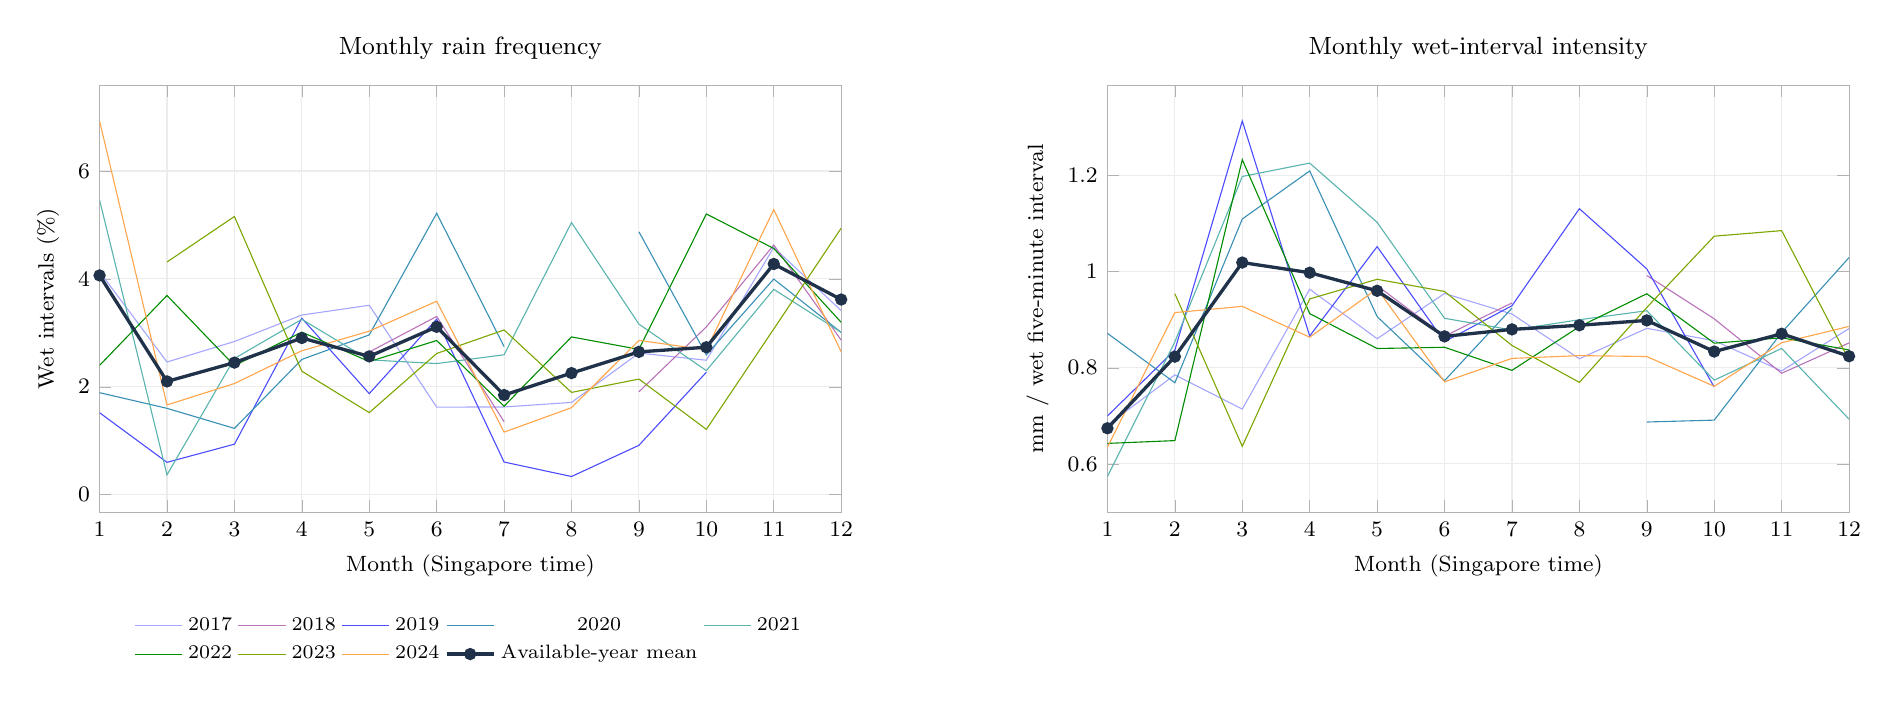
\begin{tikzpicture}
\begin{axis}[reportaxis,at={(0.0cm,0)},anchor=south west,width=11cm,height=7cm,title={Monthly rain frequency},xlabel={Month (Singapore time)},ylabel={Wet intervals (\%)},xmin=1,xmax=12,xtick={1,...,12},legend style={at={(.5,-.22)},anchor=north,legend columns=5,font=\scriptsize,draw=none}]
\addplot[blue!35,thin,unbounded coords=jump] coordinates {(1.0000000,4.1337072) (2.0000000,2.4590931) (3.0000000,2.8393303) (4.0000000,3.3304245) (5.0000000,3.5110547) (6.0000000,1.6229836) (7.0000000,1.6258171) (8.0000000,1.7099820) (9.0000000,2.6257924) (10.0000000,2.4920897) (11.0000000,4.5838666) (12.0000000,3.4117594)};
\addlegendentry{2017}
\addplot[violet!55,thin,unbounded coords=jump] coordinates {(1.0000000,6.1237253) (2.0000000,nan) (3.0000000,nan) (4.0000000,nan) (5.0000000,2.6448992) (6.0000000,3.3040671) (7.0000000,1.3533385) (8.0000000,nan) (9.0000000,1.9073088) (10.0000000,3.1106624) (11.0000000,4.6283106) (12.0000000,2.8647243)};
\addlegendentry{2018}
\addplot[blue!70,thin,unbounded coords=jump] coordinates {(1.0000000,1.5187865) (2.0000000,0.5992827) (3.0000000,0.9360135) (4.0000000,3.2711430) (5.0000000,1.8730538) (6.0000000,3.2542370) (7.0000000,0.6048855) (8.0000000,0.3364614) (9.0000000,0.9148673) (10.0000000,2.2695459) (11.0000000,nan) (12.0000000,5.8638858)};
\addlegendentry{2019}
\addplot[cyan!70!black,thin,unbounded coords=jump] coordinates {(1.0000000,1.8906216) (2.0000000,1.6004612) (3.0000000,1.2288107) (4.0000000,2.5071253) (5.0000000,2.9620978) (6.0000000,5.2163841) (7.0000000,2.7461239) (8.0000000,nan) (9.0000000,4.8734511) (10.0000000,2.5922201) (11.0000000,3.9972491) (12.0000000,3.0066723)};
\addlegendentry{2020}
\addplot[teal!65,thin,unbounded coords=jump] coordinates {(1.0000000,5.4614245) (2.0000000,0.3659526) (3.0000000,2.5245666) (4.0000000,3.2508611) (5.0000000,2.4991364) (6.0000000,2.4305083) (7.0000000,2.5937021) (8.0000000,5.0449791) (9.0000000,3.1608676) (10.0000000,2.2997356) (11.0000000,3.8061439) (12.0000000,3.0107393)};
\addlegendentry{2021}
\addplot[green!55!black,thin,unbounded coords=jump] coordinates {(1.0000000,2.3966209) (2.0000000,3.6928177) (3.0000000,2.3920085) (4.0000000,3.0133326) (5.0000000,2.4669541) (6.0000000,2.8578928) (7.0000000,1.6400855) (8.0000000,2.9245629) (9.0000000,2.6934349) (10.0000000,5.2046446) (11.0000000,4.5642923) (12.0000000,3.1948237)};
\addlegendentry{2022}
\addplot[lime!65!black,thin,unbounded coords=jump] coordinates {(1.0000000,nan) (2.0000000,4.3133747) (3.0000000,5.1570086) (4.0000000,2.2889524) (5.0000000,1.5210937) (6.0000000,2.6172394) (7.0000000,3.0535261) (8.0000000,1.8956944) (9.0000000,2.1427251) (10.0000000,1.2112493) (11.0000000,3.0717581) (12.0000000,4.9414613)};
\addlegendentry{2023}
\addplot[orange!70,thin,unbounded coords=jump] coordinates {(1.0000000,6.9282026) (2.0000000,1.6631559) (3.0000000,2.0600266) (4.0000000,2.6673383) (5.0000000,3.0313094) (6.0000000,3.5865342) (7.0000000,1.1595134) (8.0000000,1.6126284) (9.0000000,2.8598853) (10.0000000,2.6851974) (11.0000000,5.2845180) (12.0000000,2.6469772)};
\addlegendentry{2024}
\addplot[ink,very thick,mark=*,mark size=1.6pt] coordinates {(1.0000000,4.0647269) (2.0000000,2.0991625) (3.0000000,2.4482521) (4.0000000,2.9041682) (5.0000000,2.5636999) (6.0000000,3.1112308) (7.0000000,1.8471240) (8.0000000,2.2540514) (9.0000000,2.6472916) (10.0000000,2.7331681) (11.0000000,4.2765912) (12.0000000,3.6176304)};
\addlegendentry{Available-year mean}
\end{axis}
\begin{axis}[reportaxis,at={(12.8cm,0)},anchor=south west,width=11cm,height=7cm,title={Monthly wet-interval intensity},xlabel={Month (Singapore time)},ylabel={mm / wet five-minute interval},xmin=1,xmax=12,xtick={1,...,12}]
\addplot[blue!35,thin,unbounded coords=jump] coordinates {(1.0000000,0.6809519) (2.0000000,0.7853737) (3.0000000,0.7142056) (4.0000000,0.9636954) (5.0000000,0.8606764) (6.0000000,0.9548476) (7.0000000,0.9119894) (8.0000000,0.8189133) (9.0000000,0.8822372) (10.0000000,0.8565021) (11.0000000,0.7936620) (12.0000000,0.8818587)};
\addplot[violet!55,thin,unbounded coords=jump] coordinates {(1.0000000,0.6156575) (2.0000000,nan) (3.0000000,nan) (4.0000000,nan) (5.0000000,0.9710962) (6.0000000,0.8658653) (7.0000000,0.9351599) (8.0000000,nan) (9.0000000,0.9922437) (10.0000000,0.9020808) (11.0000000,0.7887351) (12.0000000,0.8519175)};
\addplot[blue!70,thin,unbounded coords=jump] coordinates {(1.0000000,0.6998529) (2.0000000,0.8370003) (3.0000000,1.3138204) (4.0000000,0.8662711) (5.0000000,1.0523488) (6.0000000,0.8545412) (7.0000000,0.9293097) (8.0000000,1.1312366) (9.0000000,1.0059431) (10.0000000,0.7601947) (11.0000000,nan) (12.0000000,0.5974865)};
\addplot[cyan!70!black,thin,unbounded coords=jump] coordinates {(1.0000000,0.8718005) (2.0000000,0.7688929) (3.0000000,1.1098208) (4.0000000,1.2098107) (5.0000000,0.9068114) (6.0000000,0.7733030) (7.0000000,0.9242406) (8.0000000,nan) (9.0000000,0.6872772) (10.0000000,0.6912090) (11.0000000,0.8734108) (12.0000000,1.0295431)};
\addplot[teal!65,thin,unbounded coords=jump] coordinates {(1.0000000,0.5738463) (2.0000000,0.8542329) (3.0000000,1.1983265) (4.0000000,1.2261795) (5.0000000,1.1029534) (6.0000000,0.9031507) (7.0000000,0.8787736) (8.0000000,0.9001390) (9.0000000,0.9188615) (10.0000000,0.7743319) (11.0000000,0.8403814) (12.0000000,0.6931660)};
\addplot[green!55!black,thin,unbounded coords=jump] coordinates {(1.0000000,0.6427524) (2.0000000,0.6485804) (3.0000000,1.2333830) (4.0000000,0.9129351) (5.0000000,0.8402641) (6.0000000,0.8428531) (7.0000000,0.7947747) (8.0000000,0.8858209) (9.0000000,0.9541984) (10.0000000,0.8513267) (11.0000000,0.8625797) (12.0000000,0.8373184)};
\addplot[lime!65!black,thin,unbounded coords=jump] coordinates {(1.0000000,nan) (2.0000000,0.9542101) (3.0000000,0.6367546) (4.0000000,0.9434971) (5.0000000,0.9843424) (6.0000000,0.9590180) (7.0000000,0.8466279) (8.0000000,0.7698636) (9.0000000,0.9256239) (10.0000000,1.0740335) (11.0000000,1.0856061) (12.0000000,0.8158447)};
\addplot[orange!70,thin,unbounded coords=jump] coordinates {(1.0000000,0.6349691) (2.0000000,0.9150161) (3.0000000,0.9279460) (4.0000000,0.8637686) (5.0000000,0.9644492) (6.0000000,0.7708670) (7.0000000,0.8196850) (8.0000000,0.8254854) (9.0000000,0.8235768) (10.0000000,0.7615814) (11.0000000,0.8522492) (12.0000000,0.8862629)};
\addplot[ink,very thick,mark=*,mark size=1.6pt] coordinates {(1.0000000,0.6742615) (2.0000000,0.8233295) (3.0000000,1.0191795) (4.0000000,0.9980225) (5.0000000,0.9603677) (6.0000000,0.8655557) (7.0000000,0.8800701) (8.0000000,0.8885765) (9.0000000,0.8987452) (10.0000000,0.8339075) (11.0000000,0.8709463) (12.0000000,0.8241747)};
\end{axis}
\end{tikzpicture}\end{center}
\vspace{5mm}\noindent Eligible station-months from the fixed panel require at least 80\% coverage, with equal averaging over stations followed by available years. Mean monthly rain frequency is highest in November (4.28\%) and lowest in July (1.85\%). Mean wet-interval amounts are about 1.02 mm in March and 0.67 mm in January. Frequency and wet-interval amount show different seasonal patterns. Each month includes 6--8 years, and each eligible year-month includes 17--21 stations.

\textbf{Task 2 features (month).} Monthly frequency and wet-interval intensity vary differently. We encode month using sine and cosine to represent the annual cycle and combine them with hour encoding to capture seasonal variation in diurnal rainfall.
\clearpage\section*{Figure 3: Annual changes in the fixed panel}

\begin{center}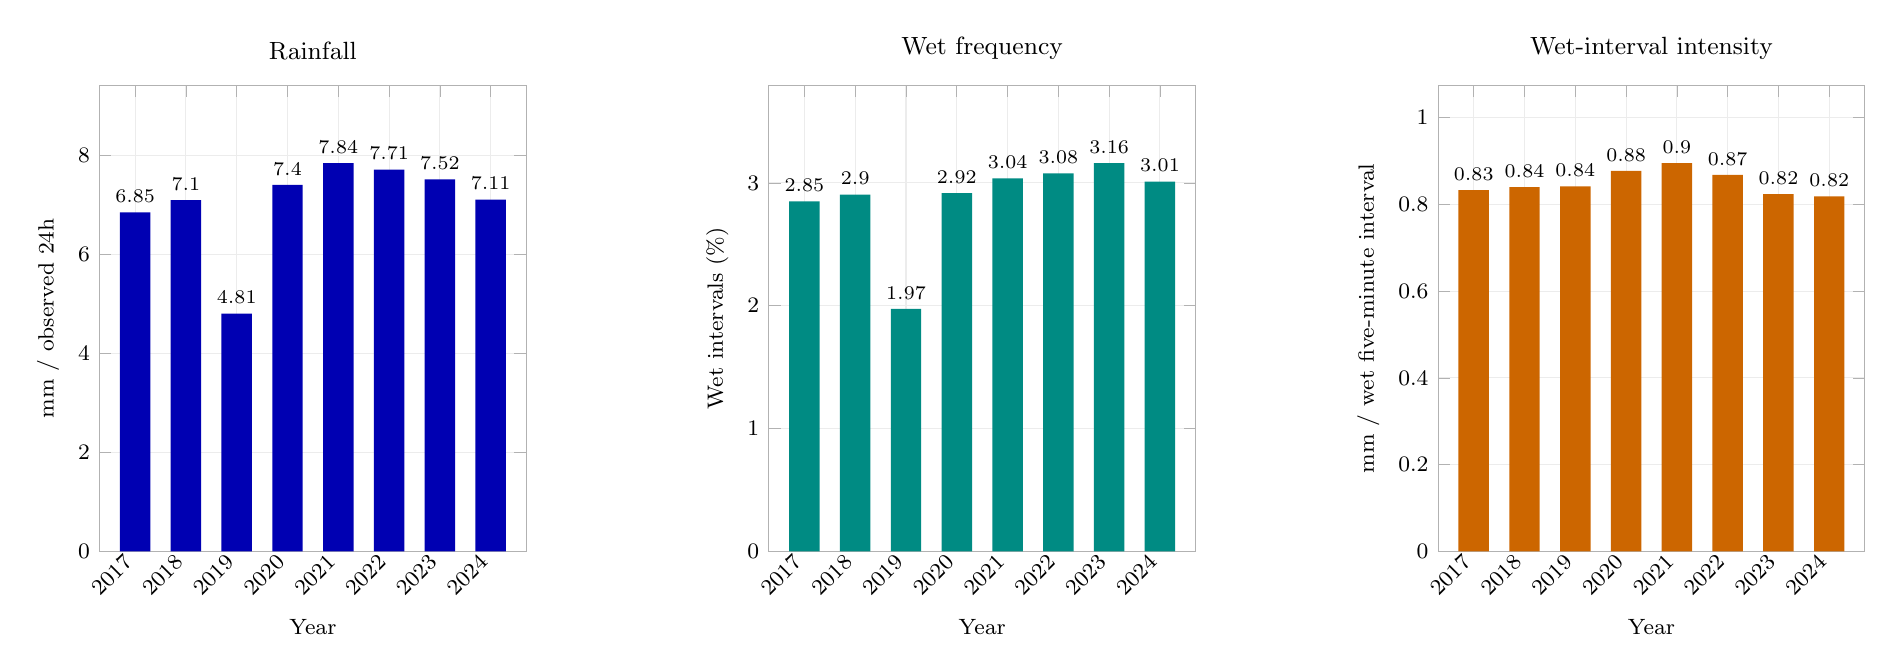
\begin{tikzpicture}
\begin{axis}[reportaxis,at={(0.0cm,0)},anchor=south west,width=7cm,height=7.5cm,title={Rainfall},xlabel={Year},ylabel={mm / observed 24h},ymin=0,ymax=9.4116,xtick={2017,...,2024},scaled ticks=false,xticklabel style={rotate=45,anchor=east},/pgf/number format/precision=2]
\addplot[ybar,fill=blue!70!black,draw=none,bar width=11pt,nodes near coords,nodes near coords style={font=\scriptsize},point meta=y] coordinates {(2017.0000000,6.8480268) (2018.0000000,7.0955196) (2019.0000000,4.8052977) (2020.0000000,7.4013320) (2021.0000000,7.8429741) (2022.0000000,7.7117387) (2023.0000000,7.5152648) (2024.0000000,7.1053278)};
\end{axis}
\begin{axis}[reportaxis,at={(8.5cm,0)},anchor=south west,width=7cm,height=7.5cm,title={Wet frequency},xlabel={Year},ylabel={Wet intervals (\%)},ymin=0,ymax=3.7934,xtick={2017,...,2024},scaled ticks=false,xticklabel style={rotate=45,anchor=east},/pgf/number format/precision=2]
\addplot[ybar,fill=teal,draw=none,bar width=11pt,nodes near coords,nodes near coords style={font=\scriptsize},point meta=y] coordinates {(2017.0000000,2.8499578) (2018.0000000,2.9040180) (2019.0000000,1.9744882) (2020.0000000,2.9172182) (2021.0000000,3.0365820) (2022.0000000,3.0770829) (2023.0000000,3.1611809) (2024.0000000,3.0107386)};
\end{axis}
\begin{axis}[reportaxis,at={(17.0cm,0)},anchor=south west,width=7cm,height=7.5cm,title={Wet-interval intensity},xlabel={Year},ylabel={mm / wet five-minute interval},ymin=0,ymax=1.0744,xtick={2017,...,2024},scaled ticks=false,xticklabel style={rotate=45,anchor=east},/pgf/number format/precision=2]
\addplot[ybar,fill=orange!80!black,draw=none,bar width=11pt,nodes near coords,nodes near coords style={font=\scriptsize},point meta=y] coordinates {(2017.0000000,0.8332878) (2018.0000000,0.8396547) (2019.0000000,0.8414619) (2020.0000000,0.8773008) (2021.0000000,0.8953600) (2022.0000000,0.8679529) (2023.0000000,0.8236592) (2024.0000000,0.8188827)};
\end{axis}
\end{tikzpicture}\end{center}
\noindent Each year compares the same 21 equally weighted stations, each with annual coverage of at least 80\%. Mean rainfall per observed 24 hours ranges from 4.81 mm in 2019 to 7.84 mm in 2021. Rain frequency in 2019 is 1.97\%, below the other years, while its wet-interval amount of 0.841 mm is close to adjacent years. Lower rainfall frequency is thus the main component associated with its lower normalized rainfall.

\textbf{Task 2 features (year).} Training, validation and test are split chronologically. Models use cyclic month and hour features without year identifiers. NEA relates the dry conditions in 2019 to a strong positive Indian Ocean Dipole, providing external context for annual variation.
\clearpage\section*{Figure 4: Diurnal variation in rainfall frequency}

\begin{center}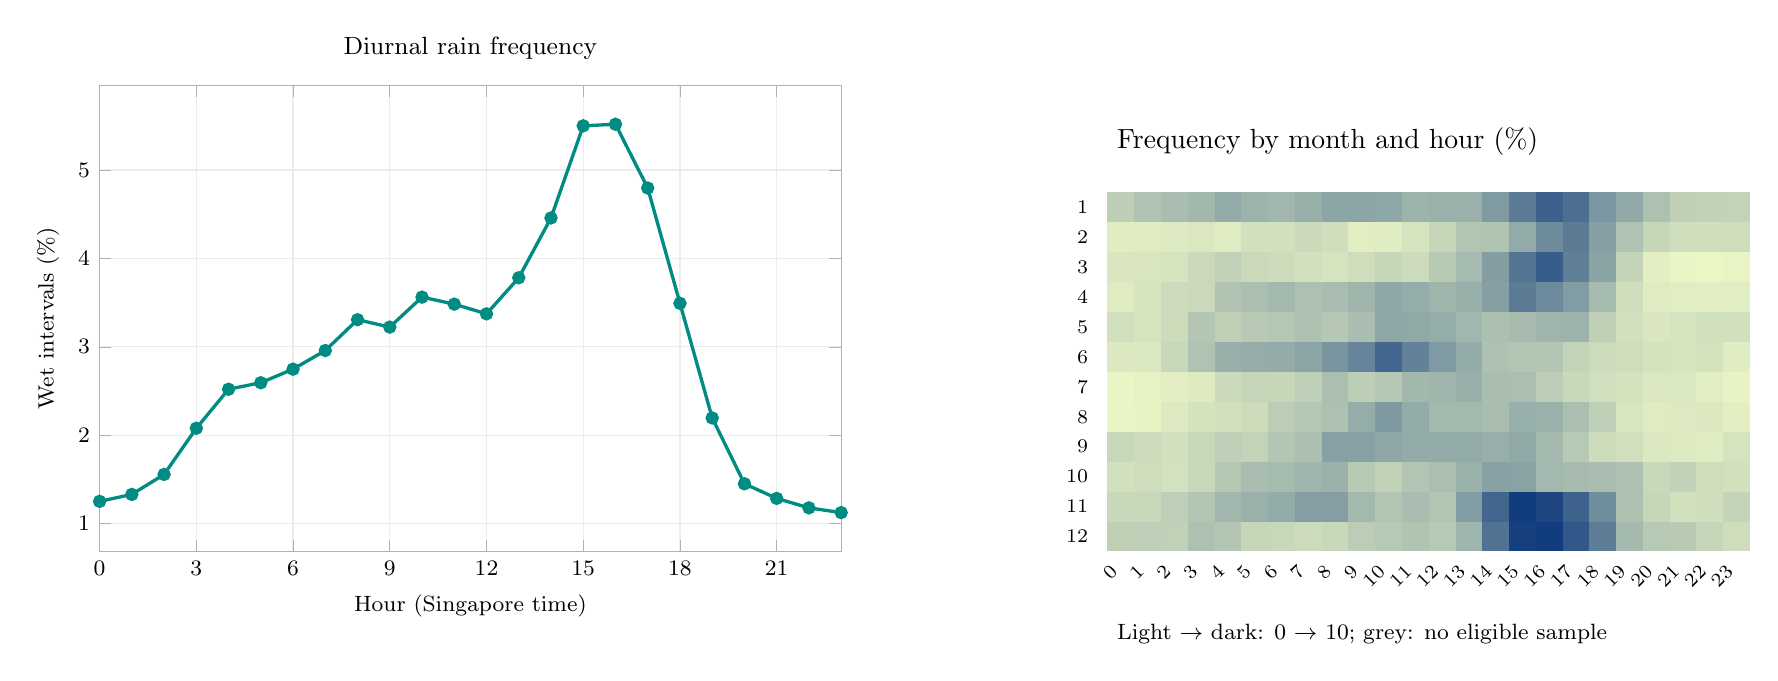
\begin{tikzpicture}
\begin{axis}[reportaxis,at={(0cm,0)},anchor=south west,width=11cm,height=7.5cm,title={Diurnal rain frequency},xlabel={Hour (Singapore time)},ylabel={Wet intervals (\%)},xtick={0,3,...,21},xmin=0,xmax=23]
\addplot[teal,very thick,mark=*,mark size=1.8pt] coordinates {(0.0000000,1.2522678) (1.0000000,1.3309341) (2.0000000,1.5568676) (3.0000000,2.0789013) (4.0000000,2.5202763) (5.0000000,2.5941759) (6.0000000,2.7472423) (7.0000000,2.9582668) (8.0000000,3.3067713) (9.0000000,3.2231866) (10.0000000,3.5621314) (11.0000000,3.4827523) (12.0000000,3.3729001) (13.0000000,3.7807871) (14.0000000,4.4575566) (15.0000000,5.4992538) (16.0000000,5.5169481) (17.0000000,4.7956033) (18.0000000,3.4919025) (19.0000000,2.1956707) (20.0000000,1.4511626) (21.0000000,1.2859725) (22.0000000,1.1787759) (23.0000000,1.1251816)};
\end{axis}
\node[anchor=west] at (12.8,5.2){Frequency by month and hour (\%)};
\begin{scope}[xshift=12.8cm]
\fill[fill={rgb,1:red,0.7389;green,0.8086;blue,0.7137}] (0.000,4.180) rectangle (0.340,4.560);
\fill[fill={rgb,1:red,0.6872;green,0.7645;blue,0.6967}] (0.340,4.180) rectangle (0.680,4.560);
\fill[fill={rgb,1:red,0.6625;green,0.7435;blue,0.6886}] (0.680,4.180) rectangle (1.020,4.560);
\fill[fill={rgb,1:red,0.6372;green,0.7219;blue,0.6802}] (1.020,4.180) rectangle (1.360,4.560);
\fill[fill={rgb,1:red,0.5732;green,0.6674;blue,0.6591}] (1.360,4.180) rectangle (1.700,4.560);
\fill[fill={rgb,1:red,0.6126;green,0.7010;blue,0.6721}] (1.700,4.180) rectangle (2.040,4.560);
\fill[fill={rgb,1:red,0.6320;green,0.7175;blue,0.6785}] (2.040,4.180) rectangle (2.380,4.560);
\fill[fill={rgb,1:red,0.5945;green,0.6855;blue,0.6661}] (2.380,4.180) rectangle (2.720,4.560);
\fill[fill={rgb,1:red,0.5473;green,0.6453;blue,0.6506}] (2.720,4.180) rectangle (3.060,4.560);
\fill[fill={rgb,1:red,0.5470;green,0.6451;blue,0.6505}] (3.060,4.180) rectangle (3.400,4.560);
\fill[fill={rgb,1:red,0.5566;green,0.6532;blue,0.6536}] (3.400,4.180) rectangle (3.740,4.560);
\fill[fill={rgb,1:red,0.6117;green,0.7002;blue,0.6718}] (3.740,4.180) rectangle (4.080,4.560);
\fill[fill={rgb,1:red,0.6049;green,0.6944;blue,0.6696}] (4.080,4.180) rectangle (4.420,4.560);
\fill[fill={rgb,1:red,0.6029;green,0.6927;blue,0.6689}] (4.420,4.180) rectangle (4.760,4.560);
\fill[fill={rgb,1:red,0.4973;green,0.6027;blue,0.6341}] (4.760,4.180) rectangle (5.100,4.560);
\fill[fill={rgb,1:red,0.3559;green,0.4822;blue,0.5875}] (5.100,4.180) rectangle (5.440,4.560);
\fill[fill={rgb,1:red,0.2356;green,0.3797;blue,0.5479}] (5.440,4.180) rectangle (5.780,4.560);
\fill[fill={rgb,1:red,0.2944;green,0.4298;blue,0.5672}] (5.780,4.180) rectangle (6.120,4.560);
\fill[fill={rgb,1:red,0.4866;green,0.5936;blue,0.6306}] (6.120,4.180) rectangle (6.460,4.560);
\fill[fill={rgb,1:red,0.5668;green,0.6620;blue,0.6570}] (6.460,4.180) rectangle (6.800,4.560);
\fill[fill={rgb,1:red,0.6797;green,0.7582;blue,0.6942}] (6.800,4.180) rectangle (7.140,4.560);
\fill[fill={rgb,1:red,0.7484;green,0.8167;blue,0.7168}] (7.140,4.180) rectangle (7.480,4.560);
\fill[fill={rgb,1:red,0.7583;green,0.8251;blue,0.7201}] (7.480,4.180) rectangle (7.820,4.560);
\fill[fill={rgb,1:red,0.7605;green,0.8270;blue,0.7209}] (7.820,4.180) rectangle (8.160,4.560);
\fill[fill={rgb,1:red,0.8767;green,0.9260;blue,0.7591}] (0.000,3.800) rectangle (0.340,4.180);
\fill[fill={rgb,1:red,0.8727;green,0.9226;blue,0.7578}] (0.340,3.800) rectangle (0.680,4.180);
\fill[fill={rgb,1:red,0.8666;green,0.9175;blue,0.7558}] (0.680,3.800) rectangle (1.020,4.180);
\fill[fill={rgb,1:red,0.8550;green,0.9076;blue,0.7520}] (1.020,3.800) rectangle (1.360,4.180);
\fill[fill={rgb,1:red,0.8755;green,0.9250;blue,0.7587}] (1.360,3.800) rectangle (1.700,4.180);
\fill[fill={rgb,1:red,0.8197;green,0.8775;blue,0.7404}] (1.700,3.800) rectangle (2.040,4.180);
\fill[fill={rgb,1:red,0.8215;green,0.8790;blue,0.7409}] (2.040,3.800) rectangle (2.380,4.180);
\fill[fill={rgb,1:red,0.7944;green,0.8559;blue,0.7320}] (2.380,3.800) rectangle (2.720,4.180);
\fill[fill={rgb,1:red,0.8129;green,0.8716;blue,0.7381}] (2.720,3.800) rectangle (3.060,4.180);
\fill[fill={rgb,1:red,0.8866;green,0.9344;blue,0.7624}] (3.060,3.800) rectangle (3.400,4.180);
\fill[fill={rgb,1:red,0.8786;green,0.9277;blue,0.7598}] (3.400,3.800) rectangle (3.740,4.180);
\fill[fill={rgb,1:red,0.8351;green,0.8906;blue,0.7454}] (3.740,3.800) rectangle (4.080,4.180);
\fill[fill={rgb,1:red,0.7749;green,0.8393;blue,0.7256}] (4.080,3.800) rectangle (4.420,4.180);
\fill[fill={rgb,1:red,0.6981;green,0.7739;blue,0.7003}] (4.420,3.800) rectangle (4.760,4.180);
\fill[fill={rgb,1:red,0.6920;green,0.7687;blue,0.6983}] (4.760,3.800) rectangle (5.100,4.180);
\fill[fill={rgb,1:red,0.5713;green,0.6657;blue,0.6585}] (5.100,3.800) rectangle (5.440,4.180);
\fill[fill={rgb,1:red,0.4305;green,0.5458;blue,0.6121}] (5.440,3.800) rectangle (5.780,4.180);
\fill[fill={rgb,1:red,0.3616;green,0.4870;blue,0.5894}] (5.780,3.800) rectangle (6.120,4.180);
\fill[fill={rgb,1:red,0.5203;green,0.6223;blue,0.6417}] (6.120,3.800) rectangle (6.460,4.180);
\fill[fill={rgb,1:red,0.6853;green,0.7629;blue,0.6961}] (6.460,3.800) rectangle (6.800,4.180);
\fill[fill={rgb,1:red,0.7779;green,0.8419;blue,0.7266}] (6.800,3.800) rectangle (7.140,4.180);
\fill[fill={rgb,1:red,0.8134;green,0.8721;blue,0.7383}] (7.140,3.800) rectangle (7.480,4.180);
\fill[fill={rgb,1:red,0.8111;green,0.8702;blue,0.7375}] (7.480,3.800) rectangle (7.820,4.180);
\fill[fill={rgb,1:red,0.8082;green,0.8677;blue,0.7366}] (7.820,3.800) rectangle (8.160,4.180);
\fill[fill={rgb,1:red,0.8504;green,0.9037;blue,0.7505}] (0.000,3.420) rectangle (0.340,3.800);
\fill[fill={rgb,1:red,0.8506;green,0.9038;blue,0.7505}] (0.340,3.420) rectangle (0.680,3.800);
\fill[fill={rgb,1:red,0.8358;green,0.8912;blue,0.7457}] (0.680,3.420) rectangle (1.020,3.800);
\fill[fill={rgb,1:red,0.7906;green,0.8527;blue,0.7308}] (1.020,3.420) rectangle (1.360,3.800);
\fill[fill={rgb,1:red,0.7573;green,0.8243;blue,0.7198}] (1.360,3.420) rectangle (1.700,3.800);
\fill[fill={rgb,1:red,0.7888;green,0.8511;blue,0.7302}] (1.700,3.420) rectangle (2.040,3.800);
\fill[fill={rgb,1:red,0.8033;green,0.8635;blue,0.7349}] (2.040,3.420) rectangle (2.380,3.800);
\fill[fill={rgb,1:red,0.8245;green,0.8816;blue,0.7419}] (2.380,3.420) rectangle (2.720,3.800);
\fill[fill={rgb,1:red,0.8334;green,0.8891;blue,0.7449}] (2.720,3.420) rectangle (3.060,3.800);
\fill[fill={rgb,1:red,0.8081;green,0.8676;blue,0.7365}] (3.060,3.420) rectangle (3.400,3.800);
\fill[fill={rgb,1:red,0.7728;green,0.8375;blue,0.7249}] (3.400,3.420) rectangle (3.740,3.800);
\fill[fill={rgb,1:red,0.7982;green,0.8592;blue,0.7333}] (3.740,3.420) rectangle (4.080,3.800);
\fill[fill={rgb,1:red,0.7185;green,0.7912;blue,0.7070}] (4.080,3.420) rectangle (4.420,3.800);
\fill[fill={rgb,1:red,0.6509;green,0.7336;blue,0.6847}] (4.420,3.420) rectangle (4.760,3.800);
\fill[fill={rgb,1:red,0.5131;green,0.6161;blue,0.6393}] (4.760,3.420) rectangle (5.100,3.800);
\fill[fill={rgb,1:red,0.3273;green,0.4578;blue,0.5781}] (5.100,3.420) rectangle (5.440,3.800);
\fill[fill={rgb,1:red,0.2162;green,0.3631;blue,0.5415}] (5.440,3.420) rectangle (5.780,3.800);
\fill[fill={rgb,1:red,0.3770;green,0.5001;blue,0.5945}] (5.780,3.420) rectangle (6.120,3.800);
\fill[fill={rgb,1:red,0.5413;green,0.6402;blue,0.6486}] (6.120,3.420) rectangle (6.460,3.800);
\fill[fill={rgb,1:red,0.7604;green,0.8269;blue,0.7208}] (6.460,3.420) rectangle (6.800,3.800);
\fill[fill={rgb,1:red,0.8895;green,0.9370;blue,0.7634}] (6.800,3.420) rectangle (7.140,3.800);
\fill[fill={rgb,1:red,0.9190;green,0.9621;blue,0.7731}] (7.140,3.420) rectangle (7.480,3.800);
\fill[fill={rgb,1:red,0.9210;green,0.9638;blue,0.7738}] (7.480,3.420) rectangle (7.820,3.800);
\fill[fill={rgb,1:red,0.9110;green,0.9553;blue,0.7705}] (7.820,3.420) rectangle (8.160,3.800);
\fill[fill={rgb,1:red,0.8758;green,0.9253;blue,0.7589}] (0.000,3.040) rectangle (0.340,3.420);
\fill[fill={rgb,1:red,0.8407;green,0.8954;blue,0.7473}] (0.340,3.040) rectangle (0.680,3.420);
\fill[fill={rgb,1:red,0.7962;green,0.8574;blue,0.7326}] (0.680,3.040) rectangle (1.020,3.420);
\fill[fill={rgb,1:red,0.7909;green,0.8529;blue,0.7308}] (1.020,3.040) rectangle (1.360,3.420);
\fill[fill={rgb,1:red,0.6941;green,0.7704;blue,0.6990}] (1.360,3.040) rectangle (1.700,3.420);
\fill[fill={rgb,1:red,0.6675;green,0.7477;blue,0.6902}] (1.700,3.040) rectangle (2.040,3.420);
\fill[fill={rgb,1:red,0.6392;green,0.7236;blue,0.6809}] (2.040,3.040) rectangle (2.380,3.420);
\fill[fill={rgb,1:red,0.6802;green,0.7586;blue,0.6944}] (2.380,3.040) rectangle (2.720,3.420);
\fill[fill={rgb,1:red,0.6587;green,0.7403;blue,0.6873}] (2.720,3.040) rectangle (3.060,3.420);
\fill[fill={rgb,1:red,0.6232;green,0.7100;blue,0.6756}] (3.060,3.040) rectangle (3.400,3.420);
\fill[fill={rgb,1:red,0.5578;green,0.6543;blue,0.6541}] (3.400,3.040) rectangle (3.740,3.420);
\fill[fill={rgb,1:red,0.5848;green,0.6773;blue,0.6630}] (3.740,3.040) rectangle (4.080,3.420);
\fill[fill={rgb,1:red,0.6228;green,0.7097;blue,0.6755}] (4.080,3.040) rectangle (4.420,3.420);
\fill[fill={rgb,1:red,0.5993;green,0.6897;blue,0.6677}] (4.420,3.040) rectangle (4.760,3.420);
\fill[fill={rgb,1:red,0.5241;green,0.6255;blue,0.6429}] (4.760,3.040) rectangle (5.100,3.420);
\fill[fill={rgb,1:red,0.3608;green,0.4863;blue,0.5891}] (5.100,3.040) rectangle (5.440,3.420);
\fill[fill={rgb,1:red,0.4245;green,0.5406;blue,0.6101}] (5.440,3.040) rectangle (5.780,3.420);
\fill[fill={rgb,1:red,0.5073;green,0.6112;blue,0.6374}] (5.780,3.040) rectangle (6.120,3.420);
\fill[fill={rgb,1:red,0.6486;green,0.7316;blue,0.6840}] (6.120,3.040) rectangle (6.460,3.420);
\fill[fill={rgb,1:red,0.8105;green,0.8697;blue,0.7373}] (6.460,3.040) rectangle (6.800,3.420);
\fill[fill={rgb,1:red,0.8751;green,0.9247;blue,0.7586}] (6.800,3.040) rectangle (7.140,3.420);
\fill[fill={rgb,1:red,0.8823;green,0.9308;blue,0.7610}] (7.140,3.040) rectangle (7.480,3.420);
\fill[fill={rgb,1:red,0.8884;green,0.9361;blue,0.7630}] (7.480,3.040) rectangle (7.820,3.420);
\fill[fill={rgb,1:red,0.8822;green,0.9307;blue,0.7610}] (7.820,3.040) rectangle (8.160,3.420);
\fill[fill={rgb,1:red,0.8149;green,0.8734;blue,0.7388}] (0.000,2.660) rectangle (0.340,3.040);
\fill[fill={rgb,1:red,0.8385;green,0.8935;blue,0.7466}] (0.340,2.660) rectangle (0.680,3.040);
\fill[fill={rgb,1:red,0.8015;green,0.8619;blue,0.7344}] (0.680,2.660) rectangle (1.020,3.040);
\fill[fill={rgb,1:red,0.7008;green,0.7761;blue,0.7012}] (1.020,2.660) rectangle (1.360,3.040);
\fill[fill={rgb,1:red,0.7491;green,0.8173;blue,0.7171}] (1.360,2.660) rectangle (1.700,3.040);
\fill[fill={rgb,1:red,0.7212;green,0.7935;blue,0.7079}] (1.700,2.660) rectangle (2.040,3.040);
\fill[fill={rgb,1:red,0.7048;green,0.7796;blue,0.7025}] (2.040,2.660) rectangle (2.380,3.040);
\fill[fill={rgb,1:red,0.6841;green,0.7619;blue,0.6957}] (2.380,2.660) rectangle (2.720,3.040);
\fill[fill={rgb,1:red,0.7120;green,0.7857;blue,0.7049}] (2.720,2.660) rectangle (3.060,3.040);
\fill[fill={rgb,1:red,0.6621;green,0.7431;blue,0.6884}] (3.060,2.660) rectangle (3.400,3.040);
\fill[fill={rgb,1:red,0.5607;green,0.6567;blue,0.6550}] (3.400,2.660) rectangle (3.740,3.040);
\fill[fill={rgb,1:red,0.5658;green,0.6611;blue,0.6567}] (3.740,2.660) rectangle (4.080,3.040);
\fill[fill={rgb,1:red,0.5857;green,0.6780;blue,0.6632}] (4.080,2.660) rectangle (4.420,3.040);
\fill[fill={rgb,1:red,0.6321;green,0.7176;blue,0.6785}] (4.420,2.660) rectangle (4.760,3.040);
\fill[fill={rgb,1:red,0.6729;green,0.7524;blue,0.6920}] (4.760,2.660) rectangle (5.100,3.040);
\fill[fill={rgb,1:red,0.6541;green,0.7363;blue,0.6858}] (5.100,2.660) rectangle (5.440,3.040);
\fill[fill={rgb,1:red,0.6199;green,0.7072;blue,0.6745}] (5.440,2.660) rectangle (5.780,3.040);
\fill[fill={rgb,1:red,0.6147;green,0.7028;blue,0.6728}] (5.780,2.660) rectangle (6.120,3.040);
\fill[fill={rgb,1:red,0.7478;green,0.8162;blue,0.7166}] (6.120,2.660) rectangle (6.460,3.040);
\fill[fill={rgb,1:red,0.8236;green,0.8808;blue,0.7416}] (6.460,2.660) rectangle (6.800,3.040);
\fill[fill={rgb,1:red,0.8497;green,0.9030;blue,0.7502}] (6.800,2.660) rectangle (7.140,3.040);
\fill[fill={rgb,1:red,0.8343;green,0.8899;blue,0.7452}] (7.140,2.660) rectangle (7.480,3.040);
\fill[fill={rgb,1:red,0.8243;green,0.8814;blue,0.7419}] (7.480,2.660) rectangle (7.820,3.040);
\fill[fill={rgb,1:red,0.8254;green,0.8823;blue,0.7422}] (7.820,2.660) rectangle (8.160,3.040);
\fill[fill={rgb,1:red,0.8633;green,0.9146;blue,0.7547}] (0.000,2.280) rectangle (0.340,2.660);
\fill[fill={rgb,1:red,0.8568;green,0.9091;blue,0.7526}] (0.340,2.280) rectangle (0.680,2.660);
\fill[fill={rgb,1:red,0.7819;green,0.8452;blue,0.7279}] (0.680,2.280) rectangle (1.020,2.660);
\fill[fill={rgb,1:red,0.6860;green,0.7635;blue,0.6963}] (1.020,2.280) rectangle (1.360,2.660);
\fill[fill={rgb,1:red,0.5947;green,0.6857;blue,0.6662}] (1.360,2.280) rectangle (1.700,2.660);
\fill[fill={rgb,1:red,0.5834;green,0.6761;blue,0.6625}] (1.700,2.280) rectangle (2.040,2.660);
\fill[fill={rgb,1:red,0.5785;green,0.6719;blue,0.6609}] (2.040,2.280) rectangle (2.380,2.660);
\fill[fill={rgb,1:red,0.5440;green,0.6425;blue,0.6495}] (2.380,2.280) rectangle (2.720,2.660);
\fill[fill={rgb,1:red,0.4755;green,0.5842;blue,0.6269}] (2.720,2.280) rectangle (3.060,2.660);
\fill[fill={rgb,1:red,0.4015;green,0.5210;blue,0.6025}] (3.060,2.280) rectangle (3.400,2.660);
\fill[fill={rgb,1:red,0.2623;green,0.4024;blue,0.5567}] (3.400,2.280) rectangle (3.740,2.660);
\fill[fill={rgb,1:red,0.3895;green,0.5108;blue,0.5986}] (3.740,2.280) rectangle (4.080,2.660);
\fill[fill={rgb,1:red,0.4994;green,0.6045;blue,0.6348}] (4.080,2.280) rectangle (4.420,2.660);
\fill[fill={rgb,1:red,0.5817;green,0.6746;blue,0.6619}] (4.420,2.280) rectangle (4.760,2.660);
\fill[fill={rgb,1:red,0.6809;green,0.7592;blue,0.6946}] (4.760,2.280) rectangle (5.100,2.660);
\fill[fill={rgb,1:red,0.6965;green,0.7725;blue,0.6998}] (5.100,2.280) rectangle (5.440,2.660);
\fill[fill={rgb,1:red,0.6999;green,0.7754;blue,0.7009}] (5.440,2.280) rectangle (5.780,2.660);
\fill[fill={rgb,1:red,0.7595;green,0.8261;blue,0.7205}] (5.780,2.280) rectangle (6.120,2.660);
\fill[fill={rgb,1:red,0.7968;green,0.8580;blue,0.7328}] (6.120,2.280) rectangle (6.460,2.660);
\fill[fill={rgb,1:red,0.8097;green,0.8689;blue,0.7370}] (6.460,2.280) rectangle (6.800,2.660);
\fill[fill={rgb,1:red,0.8308;green,0.8869;blue,0.7440}] (6.800,2.280) rectangle (7.140,2.660);
\fill[fill={rgb,1:red,0.8420;green,0.8965;blue,0.7477}] (7.140,2.280) rectangle (7.480,2.660);
\fill[fill={rgb,1:red,0.8272;green,0.8839;blue,0.7428}] (7.480,2.280) rectangle (7.820,2.660);
\fill[fill={rgb,1:red,0.8781;green,0.9272;blue,0.7596}] (7.820,2.280) rectangle (8.160,2.660);
\fill[fill={rgb,1:red,0.9154;green,0.9591;blue,0.7719}] (0.000,1.900) rectangle (0.340,2.280);
\fill[fill={rgb,1:red,0.9047;green,0.9499;blue,0.7684}] (0.340,1.900) rectangle (0.680,2.280);
\fill[fill={rgb,1:red,0.8889;green,0.9364;blue,0.7632}] (0.680,1.900) rectangle (1.020,2.280);
\fill[fill={rgb,1:red,0.8717;green,0.9218;blue,0.7575}] (1.020,1.900) rectangle (1.360,2.280);
\fill[fill={rgb,1:red,0.7931;green,0.8548;blue,0.7316}] (1.360,1.900) rectangle (1.700,2.280);
\fill[fill={rgb,1:red,0.7721;green,0.8369;blue,0.7247}] (1.700,1.900) rectangle (2.040,2.280);
\fill[fill={rgb,1:red,0.7740;green,0.8386;blue,0.7253}] (2.040,1.900) rectangle (2.380,2.280);
\fill[fill={rgb,1:red,0.7417;green,0.8110;blue,0.7146}] (2.380,1.900) rectangle (2.720,2.280);
\fill[fill={rgb,1:red,0.6681;green,0.7483;blue,0.6904}] (2.720,1.900) rectangle (3.060,2.280);
\fill[fill={rgb,1:red,0.7391;green,0.8088;blue,0.7138}] (3.060,1.900) rectangle (3.400,2.280);
\fill[fill={rgb,1:red,0.7114;green,0.7851;blue,0.7047}] (3.400,1.900) rectangle (3.740,2.280);
\fill[fill={rgb,1:red,0.6362;green,0.7211;blue,0.6799}] (3.740,1.900) rectangle (4.080,2.280);
\fill[fill={rgb,1:red,0.6266;green,0.7129;blue,0.6767}] (4.080,1.900) rectangle (4.420,2.280);
\fill[fill={rgb,1:red,0.5946;green,0.6856;blue,0.6662}] (4.420,1.900) rectangle (4.760,2.280);
\fill[fill={rgb,1:red,0.6660;green,0.7465;blue,0.6897}] (4.760,1.900) rectangle (5.100,2.280);
\fill[fill={rgb,1:red,0.6671;green,0.7474;blue,0.6901}] (5.100,1.900) rectangle (5.440,2.280);
\fill[fill={rgb,1:red,0.7336;green,0.8041;blue,0.7120}] (5.440,1.900) rectangle (5.780,2.280);
\fill[fill={rgb,1:red,0.7844;green,0.8474;blue,0.7287}] (5.780,1.900) rectangle (6.120,2.280);
\fill[fill={rgb,1:red,0.8173;green,0.8754;blue,0.7395}] (6.120,1.900) rectangle (6.460,2.280);
\fill[fill={rgb,1:red,0.8316;green,0.8876;blue,0.7443}] (6.460,1.900) rectangle (6.800,2.280);
\fill[fill={rgb,1:red,0.8534;green,0.9062;blue,0.7514}] (6.800,1.900) rectangle (7.140,2.280);
\fill[fill={rgb,1:red,0.8553;green,0.9079;blue,0.7521}] (7.140,1.900) rectangle (7.480,2.280);
\fill[fill={rgb,1:red,0.8813;green,0.9300;blue,0.7607}] (7.480,1.900) rectangle (7.820,2.280);
\fill[fill={rgb,1:red,0.9096;green,0.9541;blue,0.7700}] (7.820,1.900) rectangle (8.160,2.280);
\fill[fill={rgb,1:red,0.9154;green,0.9590;blue,0.7719}] (0.000,1.520) rectangle (0.340,1.900);
\fill[fill={rgb,1:red,0.9087;green,0.9533;blue,0.7697}] (0.340,1.520) rectangle (0.680,1.900);
\fill[fill={rgb,1:red,0.8670;green,0.9178;blue,0.7559}] (0.680,1.520) rectangle (1.020,1.900);
\fill[fill={rgb,1:red,0.8331;green,0.8889;blue,0.7448}] (1.020,1.520) rectangle (1.360,1.900);
\fill[fill={rgb,1:red,0.8231;green,0.8804;blue,0.7415}] (1.360,1.520) rectangle (1.700,1.900);
\fill[fill={rgb,1:red,0.8024;green,0.8627;blue,0.7346}] (1.700,1.520) rectangle (2.040,1.900);
\fill[fill={rgb,1:red,0.7325;green,0.8032;blue,0.7116}] (2.040,1.520) rectangle (2.380,1.900);
\fill[fill={rgb,1:red,0.7040;green,0.7788;blue,0.7022}] (2.380,1.520) rectangle (2.720,1.900);
\fill[fill={rgb,1:red,0.6767;green,0.7556;blue,0.6932}] (2.720,1.520) rectangle (3.060,1.900);
\fill[fill={rgb,1:red,0.5862;green,0.6785;blue,0.6634}] (3.060,1.520) rectangle (3.400,1.900);
\fill[fill={rgb,1:red,0.4936;green,0.5995;blue,0.6329}] (3.400,1.520) rectangle (3.740,1.900);
\fill[fill={rgb,1:red,0.5793;green,0.6726;blue,0.6611}] (3.740,1.520) rectangle (4.080,1.900);
\fill[fill={rgb,1:red,0.6404;green,0.7247;blue,0.6813}] (4.080,1.520) rectangle (4.420,1.900);
\fill[fill={rgb,1:red,0.6434;green,0.7272;blue,0.6823}] (4.420,1.520) rectangle (4.760,1.900);
\fill[fill={rgb,1:red,0.6609;green,0.7422;blue,0.6880}] (4.760,1.520) rectangle (5.100,1.900);
\fill[fill={rgb,1:red,0.5934;green,0.6846;blue,0.6658}] (5.100,1.520) rectangle (5.440,1.900);
\fill[fill={rgb,1:red,0.6073;green,0.6964;blue,0.6704}] (5.440,1.520) rectangle (5.780,1.900);
\fill[fill={rgb,1:red,0.6668;green,0.7472;blue,0.6900}] (5.780,1.520) rectangle (6.120,1.900);
\fill[fill={rgb,1:red,0.7453;green,0.8140;blue,0.7158}] (6.120,1.520) rectangle (6.460,1.900);
\fill[fill={rgb,1:red,0.8472;green,0.9009;blue,0.7494}] (6.460,1.520) rectangle (6.800,1.900);
\fill[fill={rgb,1:red,0.8754;green,0.9250;blue,0.7587}] (6.800,1.520) rectangle (7.140,1.900);
\fill[fill={rgb,1:red,0.8674;green,0.9181;blue,0.7561}] (7.140,1.520) rectangle (7.480,1.900);
\fill[fill={rgb,1:red,0.8608;green,0.9125;blue,0.7539}] (7.480,1.520) rectangle (7.820,1.900);
\fill[fill={rgb,1:red,0.8916;green,0.9388;blue,0.7641}] (7.820,1.520) rectangle (8.160,1.900);
\fill[fill={rgb,1:red,0.7787;green,0.8425;blue,0.7268}] (0.000,1.140) rectangle (0.340,1.520);
\fill[fill={rgb,1:red,0.7975;green,0.8585;blue,0.7330}] (0.340,1.140) rectangle (0.680,1.520);
\fill[fill={rgb,1:red,0.8228;green,0.8801;blue,0.7414}] (0.680,1.140) rectangle (1.020,1.520);
\fill[fill={rgb,1:red,0.7786;green,0.8425;blue,0.7268}] (1.020,1.140) rectangle (1.360,1.520);
\fill[fill={rgb,1:red,0.7448;green,0.8136;blue,0.7157}] (1.360,1.140) rectangle (1.700,1.520);
\fill[fill={rgb,1:red,0.7595;green,0.8261;blue,0.7205}] (1.700,1.140) rectangle (2.040,1.520);
\fill[fill={rgb,1:red,0.6991;green,0.7747;blue,0.7006}] (2.040,1.140) rectangle (2.380,1.520);
\fill[fill={rgb,1:red,0.6717;green,0.7513;blue,0.6916}] (2.380,1.140) rectangle (2.720,1.520);
\fill[fill={rgb,1:red,0.5266;green,0.6277;blue,0.6438}] (2.720,1.140) rectangle (3.060,1.520);
\fill[fill={rgb,1:red,0.5317;green,0.6320;blue,0.6454}] (3.060,1.140) rectangle (3.400,1.520);
\fill[fill={rgb,1:red,0.5590;green,0.6553;blue,0.6544}] (3.400,1.140) rectangle (3.740,1.520);
\fill[fill={rgb,1:red,0.5718;green,0.6662;blue,0.6587}] (3.740,1.140) rectangle (4.080,1.520);
\fill[fill={rgb,1:red,0.5793;green,0.6726;blue,0.6611}] (4.080,1.140) rectangle (4.420,1.520);
\fill[fill={rgb,1:red,0.5710;green,0.6655;blue,0.6584}] (4.420,1.140) rectangle (4.760,1.520);
\fill[fill={rgb,1:red,0.5923;green,0.6836;blue,0.6654}] (4.760,1.140) rectangle (5.100,1.520);
\fill[fill={rgb,1:red,0.5662;green,0.6614;blue,0.6568}] (5.100,1.140) rectangle (5.440,1.520);
\fill[fill={rgb,1:red,0.6464;green,0.7298;blue,0.6833}] (5.440,1.140) rectangle (5.780,1.520);
\fill[fill={rgb,1:red,0.7147;green,0.7880;blue,0.7057}] (5.780,1.140) rectangle (6.120,1.520);
\fill[fill={rgb,1:red,0.8053;green,0.8652;blue,0.7356}] (6.120,1.140) rectangle (6.460,1.520);
\fill[fill={rgb,1:red,0.8177;green,0.8758;blue,0.7397}] (6.460,1.140) rectangle (6.800,1.520);
\fill[fill={rgb,1:red,0.8591;green,0.9111;blue,0.7533}] (6.800,1.140) rectangle (7.140,1.520);
\fill[fill={rgb,1:red,0.8719;green,0.9219;blue,0.7576}] (7.140,1.140) rectangle (7.480,1.520);
\fill[fill={rgb,1:red,0.8787;green,0.9277;blue,0.7598}] (7.480,1.140) rectangle (7.820,1.520);
\fill[fill={rgb,1:red,0.8337;green,0.8894;blue,0.7450}] (7.820,1.140) rectangle (8.160,1.520);
\fill[fill={rgb,1:red,0.8191;green,0.8769;blue,0.7401}] (0.000,0.760) rectangle (0.340,1.140);
\fill[fill={rgb,1:red,0.8077;green,0.8672;blue,0.7364}] (0.340,0.760) rectangle (0.680,1.140);
\fill[fill={rgb,1:red,0.8287;green,0.8852;blue,0.7433}] (0.680,0.760) rectangle (1.020,1.140);
\fill[fill={rgb,1:red,0.7793;green,0.8430;blue,0.7270}] (1.020,0.760) rectangle (1.360,1.140);
\fill[fill={rgb,1:red,0.7064;green,0.7809;blue,0.7030}] (1.360,0.760) rectangle (1.700,1.140);
\fill[fill={rgb,1:red,0.6585;green,0.7400;blue,0.6872}] (1.700,0.760) rectangle (2.040,1.140);
\fill[fill={rgb,1:red,0.6485;green,0.7315;blue,0.6839}] (2.040,0.760) rectangle (2.380,1.140);
\fill[fill={rgb,1:red,0.6197;green,0.7070;blue,0.6744}] (2.380,0.760) rectangle (2.720,1.140);
\fill[fill={rgb,1:red,0.6067;green,0.6960;blue,0.6702}] (2.720,0.760) rectangle (3.060,1.140);
\fill[fill={rgb,1:red,0.7180;green,0.7908;blue,0.7068}] (3.060,0.760) rectangle (3.400,1.140);
\fill[fill={rgb,1:red,0.7505;green,0.8185;blue,0.7176}] (3.400,0.760) rectangle (3.740,1.140);
\fill[fill={rgb,1:red,0.6943;green,0.7706;blue,0.6990}] (3.740,0.760) rectangle (4.080,1.140);
\fill[fill={rgb,1:red,0.6704;green,0.7502;blue,0.6912}] (4.080,0.760) rectangle (4.420,1.140);
\fill[fill={rgb,1:red,0.6054;green,0.6948;blue,0.6697}] (4.420,0.760) rectangle (4.760,1.140);
\fill[fill={rgb,1:red,0.5327;green,0.6329;blue,0.6458}] (4.760,0.760) rectangle (5.100,1.140);
\fill[fill={rgb,1:red,0.5380;green,0.6374;blue,0.6475}] (5.100,0.760) rectangle (5.440,1.140);
\fill[fill={rgb,1:red,0.6387;green,0.7232;blue,0.6807}] (5.440,0.760) rectangle (5.780,1.140);
\fill[fill={rgb,1:red,0.6540;green,0.7363;blue,0.6858}] (5.780,0.760) rectangle (6.120,1.140);
\fill[fill={rgb,1:red,0.6642;green,0.7450;blue,0.6891}] (6.120,0.760) rectangle (6.460,1.140);
\fill[fill={rgb,1:red,0.6831;green,0.7611;blue,0.6954}] (6.460,0.760) rectangle (6.800,1.140);
\fill[fill={rgb,1:red,0.7841;green,0.8471;blue,0.7286}] (6.800,0.760) rectangle (7.140,1.140);
\fill[fill={rgb,1:red,0.7569;green,0.8240;blue,0.7197}] (7.140,0.760) rectangle (7.480,1.140);
\fill[fill={rgb,1:red,0.8082;green,0.8676;blue,0.7365}] (7.480,0.760) rectangle (7.820,1.140);
\fill[fill={rgb,1:red,0.8217;green,0.8792;blue,0.7410}] (7.820,0.760) rectangle (8.160,1.140);
\fill[fill={rgb,1:red,0.7850;green,0.8479;blue,0.7289}] (0.000,0.380) rectangle (0.340,0.760);
\fill[fill={rgb,1:red,0.7857;green,0.8485;blue,0.7292}] (0.340,0.380) rectangle (0.680,0.760);
\fill[fill={rgb,1:red,0.7425;green,0.8117;blue,0.7149}] (0.680,0.380) rectangle (1.020,0.760);
\fill[fill={rgb,1:red,0.6957;green,0.7718;blue,0.6995}] (1.020,0.380) rectangle (1.360,0.760);
\fill[fill={rgb,1:red,0.6330;green,0.7183;blue,0.6788}] (1.360,0.380) rectangle (1.700,0.760);
\fill[fill={rgb,1:red,0.6026;green,0.6924;blue,0.6688}] (1.700,0.380) rectangle (2.040,0.760);
\fill[fill={rgb,1:red,0.5783;green,0.6718;blue,0.6608}] (2.040,0.380) rectangle (2.380,0.760);
\fill[fill={rgb,1:red,0.5188;green,0.6210;blue,0.6412}] (2.380,0.380) rectangle (2.720,0.760);
\fill[fill={rgb,1:red,0.5188;green,0.6210;blue,0.6412}] (2.720,0.380) rectangle (3.060,0.760);
\fill[fill={rgb,1:red,0.6391;green,0.7236;blue,0.6808}] (3.060,0.380) rectangle (3.400,0.760);
\fill[fill={rgb,1:red,0.6962;green,0.7722;blue,0.6997}] (3.400,0.380) rectangle (3.740,0.760);
\fill[fill={rgb,1:red,0.6581;green,0.7398;blue,0.6871}] (3.740,0.380) rectangle (4.080,0.760);
\fill[fill={rgb,1:red,0.6951;green,0.7713;blue,0.6993}] (4.080,0.380) rectangle (4.420,0.760);
\fill[fill={rgb,1:red,0.5057;green,0.6099;blue,0.6369}] (4.420,0.380) rectangle (4.760,0.760);
\fill[fill={rgb,1:red,0.2598;green,0.4003;blue,0.5559}] (4.760,0.380) rectangle (5.100,0.760);
\fill[fill={rgb,1:red,0.0686;green,0.2373;blue,0.4928}] (5.100,0.380) rectangle (5.440,0.760);
\fill[fill={rgb,1:red,0.1138;green,0.2758;blue,0.5077}] (5.440,0.380) rectangle (5.780,0.760);
\fill[fill={rgb,1:red,0.2411;green,0.3843;blue,0.5497}] (5.780,0.380) rectangle (6.120,0.760);
\fill[fill={rgb,1:red,0.4386;green,0.5526;blue,0.6148}] (6.120,0.380) rectangle (6.460,0.760);
\fill[fill={rgb,1:red,0.6766;green,0.7555;blue,0.6932}] (6.460,0.380) rectangle (6.800,0.760);
\fill[fill={rgb,1:red,0.7727;green,0.8374;blue,0.7249}] (6.800,0.380) rectangle (7.140,0.760);
\fill[fill={rgb,1:red,0.8246;green,0.8816;blue,0.7420}] (7.140,0.380) rectangle (7.480,0.760);
\fill[fill={rgb,1:red,0.8118;green,0.8707;blue,0.7378}] (7.480,0.380) rectangle (7.820,0.760);
\fill[fill={rgb,1:red,0.7652;green,0.8310;blue,0.7224}] (7.820,0.380) rectangle (8.160,0.760);
\fill[fill={rgb,1:red,0.7490;green,0.8172;blue,0.7171}] (0.000,0.000) rectangle (0.340,0.380);
\fill[fill={rgb,1:red,0.7422;green,0.8115;blue,0.7148}] (0.340,0.000) rectangle (0.680,0.380);
\fill[fill={rgb,1:red,0.7502;green,0.8182;blue,0.7174}] (0.680,0.000) rectangle (1.020,0.380);
\fill[fill={rgb,1:red,0.6785;green,0.7572;blue,0.6938}] (1.020,0.000) rectangle (1.360,0.380);
\fill[fill={rgb,1:red,0.6993;green,0.7749;blue,0.7007}] (1.360,0.000) rectangle (1.700,0.380);
\fill[fill={rgb,1:red,0.7733;green,0.8379;blue,0.7251}] (1.700,0.000) rectangle (2.040,0.380);
\fill[fill={rgb,1:red,0.7813;green,0.8447;blue,0.7277}] (2.040,0.000) rectangle (2.380,0.380);
\fill[fill={rgb,1:red,0.7996;green,0.8603;blue,0.7337}] (2.380,0.000) rectangle (2.720,0.380);
\fill[fill={rgb,1:red,0.7844;green,0.8474;blue,0.7287}] (2.720,0.000) rectangle (3.060,0.380);
\fill[fill={rgb,1:red,0.7345;green,0.8049;blue,0.7123}] (3.060,0.000) rectangle (3.400,0.380);
\fill[fill={rgb,1:red,0.7137;green,0.7871;blue,0.7054}] (3.400,0.000) rectangle (3.740,0.380);
\fill[fill={rgb,1:red,0.6905;green,0.7673;blue,0.6978}] (3.740,0.000) rectangle (4.080,0.380);
\fill[fill={rgb,1:red,0.7131;green,0.7866;blue,0.7052}] (4.080,0.000) rectangle (4.420,0.380);
\fill[fill={rgb,1:red,0.6254;green,0.7118;blue,0.6763}] (4.420,0.000) rectangle (4.760,0.380);
\fill[fill={rgb,1:red,0.3161;green,0.4483;blue,0.5744}] (4.760,0.000) rectangle (5.100,0.380);
\fill[fill={rgb,1:red,0.0817;green,0.2485;blue,0.4972}] (5.100,0.000) rectangle (5.440,0.380);
\fill[fill={rgb,1:red,0.0665;green,0.2355;blue,0.4921}] (5.440,0.000) rectangle (5.780,0.380);
\fill[fill={rgb,1:red,0.1973;green,0.3470;blue,0.5353}] (5.780,0.000) rectangle (6.120,0.380);
\fill[fill={rgb,1:red,0.3654;green,0.4903;blue,0.5906}] (6.120,0.000) rectangle (6.460,0.380);
\fill[fill={rgb,1:red,0.6452;green,0.7288;blue,0.6829}] (6.460,0.000) rectangle (6.800,0.380);
\fill[fill={rgb,1:red,0.7132;green,0.7867;blue,0.7052}] (6.800,0.000) rectangle (7.140,0.380);
\fill[fill={rgb,1:red,0.7203;green,0.7928;blue,0.7076}] (7.140,0.000) rectangle (7.480,0.380);
\fill[fill={rgb,1:red,0.7721;green,0.8369;blue,0.7247}] (7.480,0.000) rectangle (7.820,0.380);
\fill[fill={rgb,1:red,0.8065;green,0.8662;blue,0.7360}] (7.820,0.000) rectangle (8.160,0.380);
\node[font=\scriptsize,rotate=45,anchor=east] at (0.170,-0.13){0};
\node[font=\scriptsize,rotate=45,anchor=east] at (0.510,-0.13){1};
\node[font=\scriptsize,rotate=45,anchor=east] at (0.850,-0.13){2};
\node[font=\scriptsize,rotate=45,anchor=east] at (1.190,-0.13){3};
\node[font=\scriptsize,rotate=45,anchor=east] at (1.530,-0.13){4};
\node[font=\scriptsize,rotate=45,anchor=east] at (1.870,-0.13){5};
\node[font=\scriptsize,rotate=45,anchor=east] at (2.210,-0.13){6};
\node[font=\scriptsize,rotate=45,anchor=east] at (2.550,-0.13){7};
\node[font=\scriptsize,rotate=45,anchor=east] at (2.890,-0.13){8};
\node[font=\scriptsize,rotate=45,anchor=east] at (3.230,-0.13){9};
\node[font=\scriptsize,rotate=45,anchor=east] at (3.570,-0.13){10};
\node[font=\scriptsize,rotate=45,anchor=east] at (3.910,-0.13){11};
\node[font=\scriptsize,rotate=45,anchor=east] at (4.250,-0.13){12};
\node[font=\scriptsize,rotate=45,anchor=east] at (4.590,-0.13){13};
\node[font=\scriptsize,rotate=45,anchor=east] at (4.930,-0.13){14};
\node[font=\scriptsize,rotate=45,anchor=east] at (5.270,-0.13){15};
\node[font=\scriptsize,rotate=45,anchor=east] at (5.610,-0.13){16};
\node[font=\scriptsize,rotate=45,anchor=east] at (5.950,-0.13){17};
\node[font=\scriptsize,rotate=45,anchor=east] at (6.290,-0.13){18};
\node[font=\scriptsize,rotate=45,anchor=east] at (6.630,-0.13){19};
\node[font=\scriptsize,rotate=45,anchor=east] at (6.970,-0.13){20};
\node[font=\scriptsize,rotate=45,anchor=east] at (7.310,-0.13){21};
\node[font=\scriptsize,rotate=45,anchor=east] at (7.650,-0.13){22};
\node[font=\scriptsize,rotate=45,anchor=east] at (7.990,-0.13){23};
\node[font=\scriptsize,anchor=east] at (-0.12,4.370){1};
\node[font=\scriptsize,anchor=east] at (-0.12,3.990){2};
\node[font=\scriptsize,anchor=east] at (-0.12,3.610){3};
\node[font=\scriptsize,anchor=east] at (-0.12,3.230){4};
\node[font=\scriptsize,anchor=east] at (-0.12,2.850){5};
\node[font=\scriptsize,anchor=east] at (-0.12,2.470){6};
\node[font=\scriptsize,anchor=east] at (-0.12,2.090){7};
\node[font=\scriptsize,anchor=east] at (-0.12,1.710){8};
\node[font=\scriptsize,anchor=east] at (-0.12,1.330){9};
\node[font=\scriptsize,anchor=east] at (-0.12,0.950){10};
\node[font=\scriptsize,anchor=east] at (-0.12,0.570){11};
\node[font=\scriptsize,anchor=east] at (-0.12,0.190){12};
\node[font=\footnotesize,anchor=west] at (0,-1.05){Light $\rightarrow$ dark: 0 $\rightarrow$ 10; grey: no eligible sample};
\end{scope}
\end{tikzpicture}\end{center}
\noindent Rain frequency peaks at 16:00--17:00, with peak timing and strength varying by month. The afternoon peak is more pronounced in November--December, while June has elevated frequency from morning toward midday. Statistics equally weight eligible station-year-month-hour strata with at least 80\% coverage. These findings motivate hour, month and their interactions as predictors.

\textbf{Task 2 feature implications (hour and month).} Encode Singapore local hour cyclically and consider month--hour interactions: the strength and timing of the afternoon peak vary by month. Logistic regression and linear SVM need explicit interaction features; trees can learn such combinations. Their predictive contribution must still be tested by ablation.
\clearpage\section*{Figure 5: Distance and daily-rainfall correlation}
\begin{center}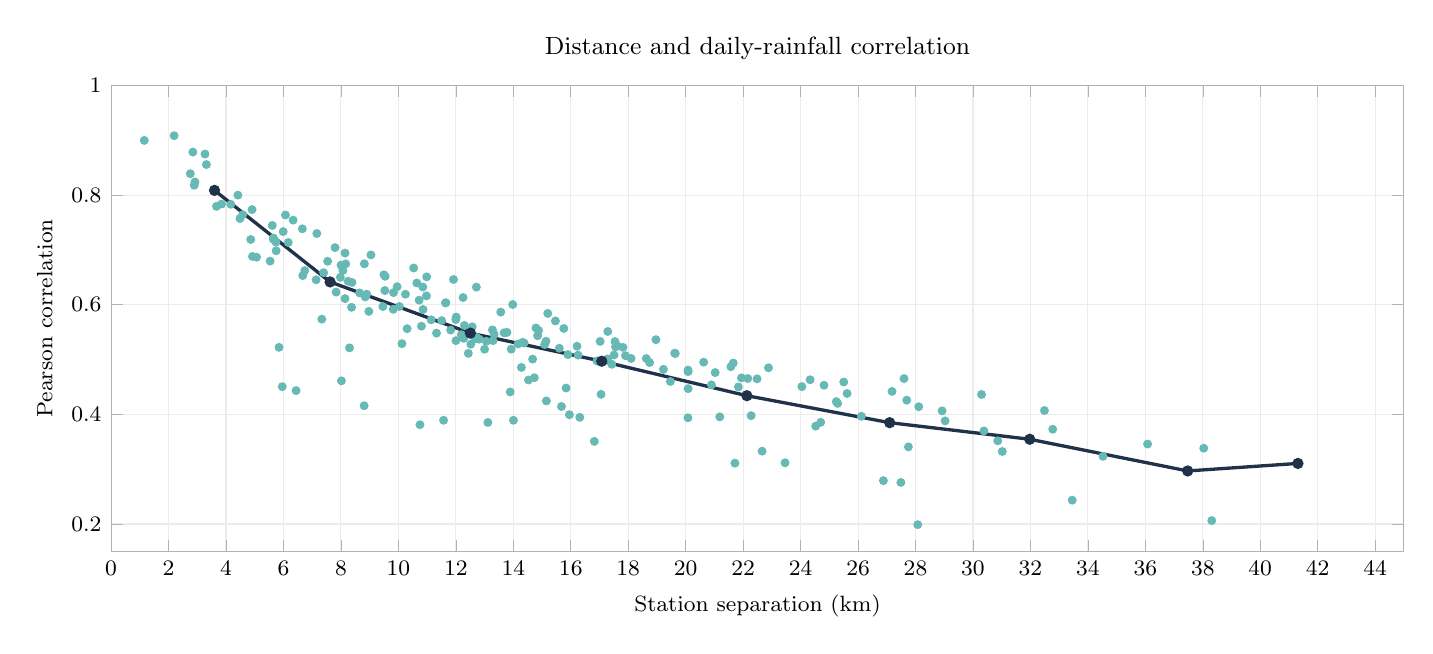
\begin{tikzpicture}
\begin{axis}[reportaxis,at={(0cm,0)},anchor=south west,width=18cm,height=7.5cm,title={Distance and daily-rainfall correlation},xlabel={Station separation (km)},ylabel={Pearson correlation},ymin=.15,ymax=1,xmin=0,xmax=45]
\addplot[teal!60,only marks,mark=*,mark size=1.4pt] coordinates {(16.3144845,0.3945964) (11.6529995,0.6034656) (10.8499077,0.6322975) (24.7007722,0.3855147) (12.8137665,0.5371191) (8.8449289,0.6141890) (11.6384330,0.6033873) (17.2877678,0.5511815) (14.7302517,0.4668321) (5.6484582,0.7191865) (7.5370720,0.6792134) (8.6489390,0.6215144) (9.9559917,0.6328810) (7.8311900,0.6230487) (9.8282122,0.6220925) (3.8450307,0.7835084) (19.2253438,0.4820845) (5.7402487,0.7141407) (6.6714693,0.6531088) (13.9799453,0.6002895) (5.8441071,0.5222734) (26.8826547,0.2791045) (38.3118019,0.2062744) (23.4582341,0.3116489) (10.7503274,0.3810825) (27.4908216,0.2758420) (6.4380603,0.4433303) (28.0757933,0.1987852) (21.7139203,0.3110013) (8.8076340,0.4157720) (16.8196412,0.3507105) (8.0173871,0.4611185) (14.0050583,0.3892141) (11.5726375,0.3891829) (13.1144559,0.3851883) (33.4549479,0.2434926) (15.9533019,0.3993911) (15.1505556,0.4244834) (5.9583556,0.4505206) (21.6563253,0.4935873) (32.4879796,0.4069937) (17.6157895,0.5248874) (4.9063704,0.7735029) (22.1606234,0.4654315) (10.5313650,0.6670193) (22.2783915,0.3975905) (17.2864195,0.5011764) (4.4856976,0.7571691) (10.9755670,0.6161670) (2.1941578,0.9082521) (8.1653985,0.6743863) (10.7222447,0.6082740) (8.0019109,0.6720844) (27.6957390,0.4257685) (10.2459829,0.6190871) (12.6817249,0.5380421) (8.1432809,0.6942311) (15.6767889,0.4143648) (11.3269864,0.5481248) (17.5400779,0.5328242) (1.1545815,0.8996528) (28.1125137,0.4139005) (8.2982933,0.5212653) (7.1613384,0.7298819) (18.0994544,0.5020237) (13.2738214,0.5540804) (19.6174055,0.5115817) (14.8442985,0.5434927) (20.0823437,0.4808144) (13.7785921,0.5494719) (10.1249996,0.5289399) (11.9983477,0.5729873) (15.9009378,0.5090766) (24.8146062,0.4530845) (15.1376366,0.5332814) (27.6000441,0.4652565) (14.5281238,0.4626376) (41.3113739,0.3104956) (10.3034515,0.5562587) (22.6599763,0.3328515) (30.3808163,0.3697846) (21.5740998,0.4869519) (30.2998062,0.4362458) (24.3310522,0.4631149) (34.5259282,0.3234714) (26.1155324,0.3964715) (5.6090894,0.7445391) (22.4847923,0.4647901) (30.8629895,0.3516897) (38.0327540,0.3382437) (12.7143637,0.6320318) (10.8021929,0.5608248) (27.1835263,0.4418289) (5.7450469,0.6983523) (14.2813628,0.4856319) (16.2520753,0.5080679) (6.6548214,0.7384542) (15.4663803,0.5703799) (9.4973017,0.6545719) (21.9404892,0.4665683) (12.5191257,0.5278913) (11.1411496,0.5724858) (8.3857772,0.6405752) (19.4670825,0.4599357) (24.0447003,0.4506049) (17.9056076,0.5069860) (14.8786388,0.5529422) (17.4262534,0.4913612) (14.3281205,0.5313997) (4.9209551,0.6879864) (6.0693814,0.7636105) (2.7571527,0.8389324) (3.2690875,0.8748412) (12.2754222,0.5386651) (5.0628533,0.6866422) (22.8824636,0.4849431) (5.6489574,0.7216685) (12.4338924,0.5112105) (12.0126225,0.5774929) (28.9257147,0.4063485) (7.3347509,0.5735901) (8.2494438,0.6427493) (18.7442748,0.4945323) (13.3322130,0.5461313) (20.0835634,0.4779711) (15.0897866,0.5272957) (21.0273208,0.4762153) (14.3770910,0.5300901) (8.9711712,0.5878010) (12.2971173,0.5621472) (16.9105658,0.4973139) (25.6183165,0.4380540) (31.0220551,0.3322423) (21.8347449,0.4500945) (10.9854921,0.6508385) (20.6263473,0.4951571) (12.2513968,0.6131051) (17.8163483,0.5222235) (9.0447492,0.6908597) (15.1988722,0.5841143) (36.0776890,0.3458413) (18.9649276,0.5362576) (13.5621610,0.5865330) (3.3174398,0.8556244) (13.8924618,0.4408666) (20.0789841,0.3937641) (11.5064963,0.5710213) (20.0847086,0.4468712) (14.1662282,0.5283960) (24.5248385,0.3785366) (15.8374450,0.4479854) (5.5346219,0.6795470) (12.1897002,0.5453457) (21.1875735,0.3954433) (27.7531807,0.3406837) (13.0596223,0.5332192) (12.5693036,0.5597216) (15.6015244,0.5205349) (12.7164390,0.5406368) (13.2937458,0.5344874) (9.4591102,0.5967003) (17.0543590,0.4364752) (10.0351000,0.5967595) (8.8980711,0.6191576) (18.6301744,0.5017963) (9.8214365,0.5916034) (3.6688756,0.7793796) (7.1366450,0.6454317) (7.3981801,0.6584071) (4.4131090,0.7999095) (25.2419437,0.4232729) (7.9795738,0.6499277) (8.3694116,0.5952401) (7.7950215,0.7041677) (8.8153742,0.6746132) (2.8450856,0.8784098) (16.2170662,0.5242857) (6.7406649,0.6622531) (17.0229071,0.5330789) (2.9180933,0.8239318) (14.6717071,0.5007159) (17.5567365,0.5231900) (5.9895968,0.7332962) (10.8574462,0.5913587) (6.1661427,0.7135319) (25.5023787,0.4590083) (8.0685387,0.6622289) (12.0047267,0.5344478) (9.5388949,0.6518306) (13.9270765,0.5189383) (4.8598997,0.7189705) (19.6379567,0.5110257) (2.8934809,0.8178634) (12.9995663,0.5187741) (14.7875722,0.5575913) (9.5283762,0.6258139) (29.0298734,0.3880837) (13.6800804,0.5487818) (4.5796101,0.7643339) (6.3359061,0.7542924) (20.8961948,0.4537686) (4.1654533,0.7831248) (8.1417199,0.6111612) (11.9177396,0.6459948) (17.5065325,0.5082991) (25.2880797,0.4199436) (32.7765854,0.3728123) (11.8190185,0.5537625) (15.7584376,0.5566300) (10.6403714,0.6396178)};
\addplot[ink,very thick,mark=*,mark size=1.4pt] coordinates {(3.5996518,0.8085525) (7.6231205,0.6415685) (12.5063802,0.5481465) (17.0768834,0.4969552) (22.1302944,0.4340133) (27.1010742,0.3848235) (31.9763885,0.3545916) (37.4740816,0.2967865) (41.3113739,0.3104956)};
\end{axis}
\end{tikzpicture}\end{center}
\noindent The 21 stations form 210 pairs. The mean Pearson correlation of daily rainfall is 0.809 for 17 pairs separated by at most 5 km, compared with 0.336 for 12 pairs more than 30 km apart. Mean correlations in 5 km distance groups generally decrease with separation, indicating spatial dependence.

\textbf{Stations are not independent.} Nearby gauges may experience the same rainfall event, and different pairs can share a station. Thus, 91 gauges are not 91 independent weather samples, and the 210 correlations are not 210 independent samples. Shared-day screening follows the criteria given earlier.

\textbf{Task 2 features (neighbours).} Stronger daily-rainfall correlation among nearby stations motivates mean rainfall, maximum rainfall and wet fractions from the three closest stations. Task 2 compares models before and after adding neighbour features to evaluate their contribution to half-hour prediction.

\clearpage\section*{Figure 6: Rainfall distribution, half-hour exceedance and persistence}

\begin{center}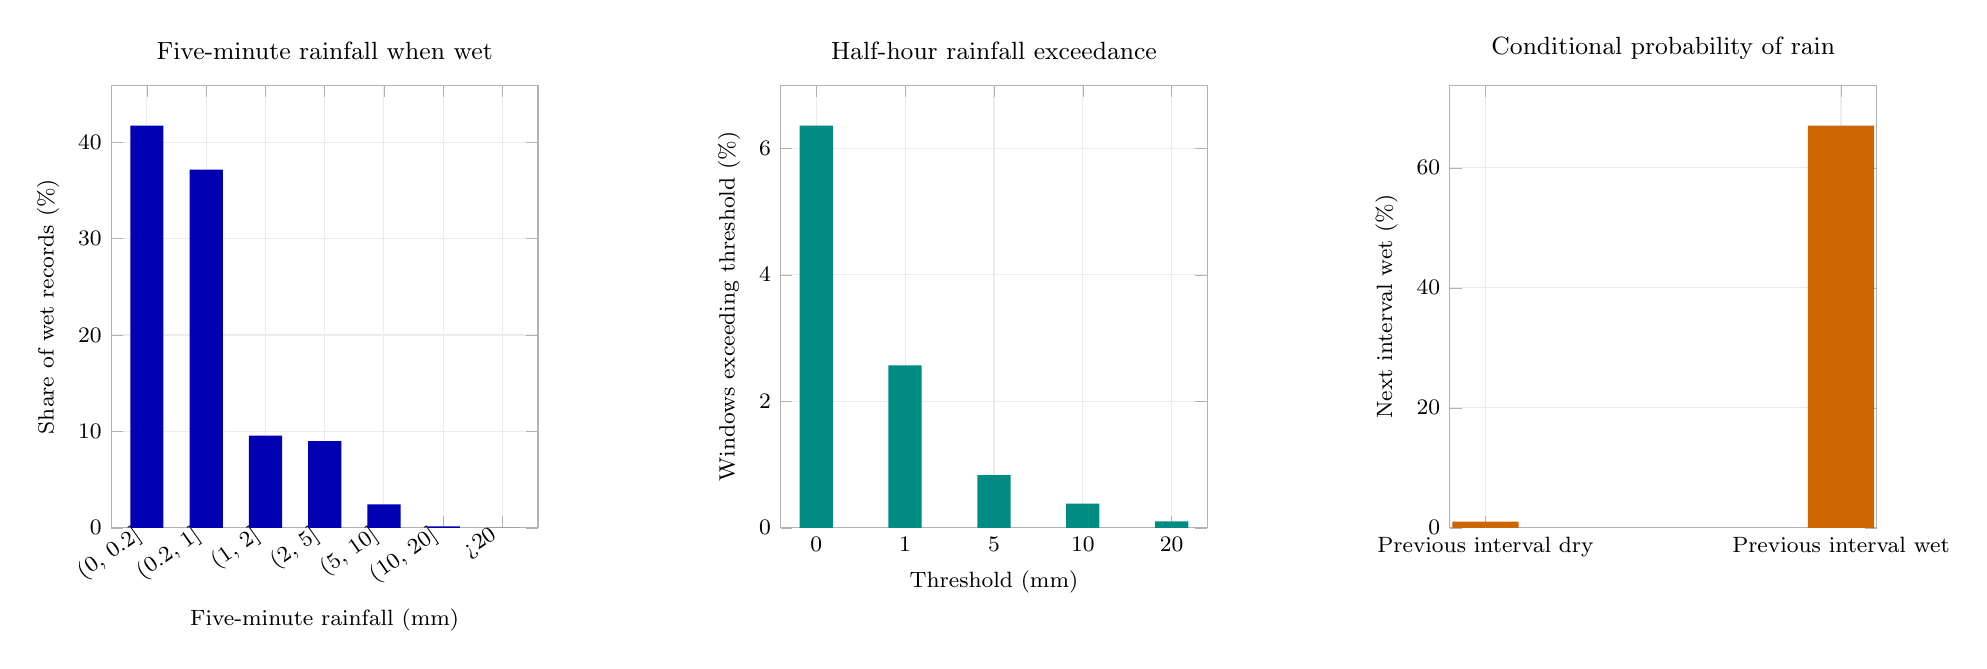
\begin{tikzpicture}
\begin{axis}[reportaxis,at={(0cm,0)},anchor=south west,width=7cm,height=7.2cm,title={Five-minute rainfall when wet},xlabel={Five-minute rainfall (mm)},ylabel={Share of wet records (\%)},xtick={0,1,2,3,4,5,6},xticklabels={{(0, 0.2]},{(0.2, 1]},{(1, 2]},{(2, 5]},{(5, 10]},{(10, 20]},{>20}},xticklabel style={rotate=35,anchor=east},ymin=0]
\addplot[ybar,fill=blue!70!black,draw=none,bar width=12pt] coordinates {(0.0000000,41.7152677) (1.0000000,37.1621336) (2.0000000,9.5575802) (3.0000000,8.9957515) (4.0000000,2.4250166) (5.0000000,0.1435447) (6.0000000,0.0007057)};
\end{axis}
\begin{axis}[reportaxis,at={(8.5cm,0)},anchor=south west,width=7cm,height=7.2cm,title={Half-hour rainfall exceedance},xlabel={Threshold (mm)},ylabel={Windows exceeding threshold (\%)},xtick={0,...,4},xticklabels={0,1,5,10,20},ymin=0]
\addplot[ybar,fill=teal,draw=none,bar width=12pt] coordinates {(0.0000000,6.3602091) (1.0000000,2.5694661) (2.0000000,0.8344686) (3.0000000,0.3816784) (4.0000000,0.1027535)};
\end{axis}
\begin{axis}[reportaxis,at={(17cm,0)},anchor=south west,width=7cm,height=7.2cm,title={Conditional probability of rain},ylabel={Next interval wet (\%)},xtick={0,1},xticklabels={Previous interval dry,Previous interval wet},ymin=0]
\addplot[ybar,fill=orange!80!black,draw=none,bar width=24pt] coordinates {(0.0000000,1.0369391) (1.0000000,67.0312500)};
\end{axis}
\end{tikzpicture}\end{center}
\noindent \textbf{Rainfall distribution in wet intervals.} Across all stations and eight years, 41.72\% of wet five-minute observations fall in $(0,0.2]$ mm and 37.16\% in $(0.2,1]$ mm. Together, 78.88\% have at most 1 mm, indicating small accumulations in most wet intervals. Dry intervals account for 97.08\% of all valid five-minute observations.

\textbf{Exceedance probability of half-hour rainfall.} There are 6,374,476 complete future six-interval windows in 2024. Subsequent 30-minute totals strictly exceed 0 mm in 6.36\% of windows and 5 mm in 0.83\%; exceedance becomes less frequent as the rainfall threshold rises. Totals are compared at nine decimal places to avoid floating-point errors at threshold boundaries. The horizontal axis uses threshold categories.

\textbf{Rainfall persistence in consecutive intervals.} For consecutive five-minute observations at the same station in 2024, the probability of rain is 1.04\% following a dry interval and 67.03\% following a wet interval. This substantial short-term persistence supports recent rainfall and wet-spell duration as predictors.

\textbf{Task 2 feature implications (persistence and rare events).} Implemented features include the latest reading, 15/30/60-minute totals, recent rainfall changes and wet-spell duration. Only records available at prediction time are used; missing readings are not dry readings. The following sections report positive counts, PR-AUC, Brier score and calibration curves separately by threshold.
\clearpage\section*{4. Task 2: target and chronological splits}
\textbf{Prediction target.} For station $s$, time $t$ and rainfall threshold $q$, estimate the probability that rainfall in the next 30 minutes strictly exceeds $q$. Use $q\in\{0,5,25\}$ mm and one classifier per target, with one feature row and three label columns per station/time.

\[R_{s,t}^{30}=\sum_{k=1}^{6}r_{s,t+5k\,\mathrm{min}},\qquad y_{s,t}^{(q)}=\mathbf{1}(R_{s,t}^{30}>q),\qquad \hat p_q=P(y^{(q)}=1\mid x_{s,t}).\]
\textbf{Label construction.} Treat timestamps as five-minute interval ends. Sum six valid intervals in $(t,t+30\mathrm{min}]$ and round to nine decimal places before comparison. Exclude the current interval and reject windows missing any future interval. Equality with the threshold is negative.

\begin{center}\begin{tabular}{lrrrr}\toprule
Purpose & Rows & $>0$ positives & $>5$ positives & $>25$ positives\\\midrule
2017--2022: all training records & 34,542,285 & 2,074,430 & 279,801 & 19,787\\
2023 H1: calibration & 3,325,499 & 251,794 & 30,699 & 1,532\\
2023 H2: selection & 3,393,373 & 197,358 & 28,000 & 2,487\\
2024: test & 6,374,476 & 405,430 & 53,193 & 3,517\\
\bottomrule\end{tabular}\end{center}

\textbf{Training and validation.} All classifiers and preprocessing use all 34,542,285 eligible 2017--2022 training records. Fit calibration on 2023 H1, select models and decision cutoffs on H2, and test on 2024. Label windows cannot cross these boundaries. Calibration, selection and test preserve natural class proportions.

\clearpage\section*{5. From Task 1 to feature engineering}
\begingroup\small
\begin{center}\begin{tabular}{p{5.2cm}p{9.0cm}p{9.0cm}}\toprule
Task 1 finding & Construction & Inputs\\\midrule
Afternoon peak varies by month & Cyclic hour/month and interactions & 8 calendar features; no year ID\\
Station differences and spatial correlation & Station ID, coordinates, three closest neighbours & Neighbour rain means, maxima and wet fractions\\
Short-term persistence & Latest reading and 5/10/15/30/60-minute lags & 15/30/60-minute totals, changes and wet-spell length\\
\bottomrule\end{tabular}\end{center}

\textbf{History and neighbours.} Use only observations available by prediction time: both observation and retained update timestamps must be no later than $t$. Search the past 90 minutes; mark the latest reading unavailable after 30 minutes. Use coordinates known by $t$ to identify three closest eligible neighbours and aggregate rainfall, available counts, ages and distances. Spark windows and joins process all records.

\textbf{Cyclic time encoding.} Let $h$ be local hour including fractional minutes and $m$ the month. Use the cyclic encodings below and their four pairwise products, giving eight features. Adjacent 23:00/00:00 and December/January stay close in feature space.

\[h_{\sin}=\sin(2\pi h/24),\quad h_{\cos}=\cos(2\pi h/24),\qquad m_{\sin}=\sin[2\pi(m-1)/12],\quad m_{\cos}=\cos[2\pi(m-1)/12].\]
\textbf{Input processing.} Fit imputation, missingness indicators and station vocabulary on the complete training period only. Use one-hot station encoding for linear models and a categorical index for trees; exclude constant features. Logistic and SVM standardize features. Nine logistic models compare calendar/station, added own history, and added neighbour history.

\textbf{Feature comparison settings.} The nine ablation classifiers use L2 parameter 0.001, at most 80 iterations and tolerance $10^{-6}$. 0 reach this iteration cap. Logistic and SVM in the main algorithm comparison allow 100 iterations.

\textbf{Feature dimensions.} The complete input has 45 numeric features and 27 missingness indicators. With station encoding, linear models have 162 dimensions and tree models 73.

\begin{center}\begin{tabular}{lrrr}\toprule
L2 logistic features & Test PR-AUC: 0 mm & 5 mm & 25 mm\\\midrule
Calendar/station & 0.11588 & 0.01671 & 0.00139\\
Add own history & 0.53158 & 0.15868 & 0.01482\\
Add neighbours & 0.56134 & 0.17982 & 0.01713\\
\bottomrule\end{tabular}\end{center}

\textbf{Neighbour contribution.} Adding neighbour history changes test PR-AUC by +0.02975, +0.02114, +0.00231 relative to own-history models, consistent with Task 1 spatial correlations.

\endgroup
\clearpage\section*{6. Models, imbalance and calibration}
\begin{center}\begin{tabular}{p{6cm}p{17cm}}\toprule
Model & Parameters\\\midrule
L2 logistic (MLlib) & $\lambda=0.001$, standardization, 100 iterations, tolerance $10^{-6}$\\
Linear SVM (MLlib) & $\lambda=0.001$, standardization, 100 iterations, tolerance $10^{-6}$\\
XGBoost (Spark interface) & 80 trees, depth 4, learning rate 0.1, 64 bins, child weight 20; $L_2=1$\\
\bottomrule\end{tabular}\end{center}

\textbf{Training policies.} Compare natural distribution, balanced weighting and constrained SMOTE. Weights are $w_+=N/(2P)$ and $w_-=N/[2(N-P)]$. SMOTE targets 20\% positives and caps their total at ten times the original count. Every policy retains all real training observations; synthetic rows enter training only.

\textbf{SMOTE construction.} All training positives are available as donors, processed sequentially by station to bound memory. Search up to five neighbours with identical station, missingness, discrete profile and rain-zero pattern. Interpolate 16 continuous rain features with one coefficient, preserving calendar and discrete information; copy isolated donors.

\textbf{Probability calibration.} Fit Platt calibration $\hat p=1/[1+\exp(-(az+b))]$ on 2023 H1, where $z$ is the base score and $a\geq0$. This converts SVM scores to probabilities and adjusts weighting/resampling probability scales. A group predicted near 10\% should ideally contain about 10\% actual positives.

\clearpage\section*{7. Evaluation and validation selection}
\textbf{Evaluation metrics.} ROC-AUC measures ranking, with random-ranking reference 0.5. PR-AUC combines precision and recall and is useful for rare positives; random-ranking precision is approximately prevalence $\pi$. Spark integrates both areas exactly. Brier score is mean squared probability error; lower is better.

\textbf{Model selection.} Compare policies for each algorithm/threshold on 2023 H2, select primarily by PR-AUC and break ties with Brier. Choose decision cutoffs by validation F1 for test precision, recall, F1 and accuracy; these differ from rainfall thresholds defining labels. Test results do not select models.

\textbf{Experiment note.} Prediction experiments are being estimated on the complete training data; this draft does not report unfinished model evaluations.

\clearpage\section*{10. AI use and references}

\textbf{AI-use declaration.} We use OpenAI Codex to assist study design, data-processing and model code, result checks and report editing. Reported rainfall statistics and model evaluations come from actual processing and model runs; SMOTE examples are used only for training.

\textbf{Sources.}
\begin{enumerate}
\item NEA, \href{https://data.gov.sg/collections/2279/view}{Historical Rainfall across Singapore}, annual datasets 2017--2024.
\item Meteorological Service Singapore, \href{https://www.weather.gov.sg/climate-climate-of-singapore}{Climate of Singapore}.
\item NEA, \href{https://www.nea.gov.sg/media/news/news/index/2019-is-singapore-s-joint-warmest-year-on-record}{Review of the climate in 2019}. External context on dry conditions and the positive Indian Ocean Dipole, not an input feature in the proposed model.
\item geoBoundaries, \href{https://www.geoboundaries.org/api/current/gbOpen/SGP/ADM0/}{Singapore ADM0}, based on URA 2016 data, ODbL 1.0.
\item Apache Spark 3.5.8, \href{https://spark.apache.org/docs/3.5.8/ml-classification-regression.html}{MLlib classification and regression documentation}, for logistic and linear SVM implementation. Evaluation uses Spark BinaryClassificationEvaluator.
\item XGBoost, \href{https://xgboost.readthedocs.io/en/release_3.2.0/tutorials/spark_estimator.html}{PySpark estimator documentation}, for external Spark integration; the actual installed version is 3.2.0.
\item scikit-learn, \href{https://scikit-learn.org/stable/modules/generated/sklearn.metrics.PrecisionRecallDisplay.html}{Precision--Recall documentation} and \href{https://scikit-learn.org/stable/modules/calibration.html}{probability-calibration documentation}.
\end{enumerate}

\end{document}
